\documentclass[12pt,a4paper]{article}
\usepackage[top=2.7cm, bottom=2cm, left=2cm, right=2cm]{geometry}
\usepackage[utf8]{inputenc}
\usepackage{CJKutf8}
\usepackage{enumitem}
\usepackage{verbatim}


%% Useful packages
\usepackage{amsmath,amssymb}
% \usepackage{subfigure}
\usepackage{graphicx,wrapfig}
\usepackage[dvipsnames,table]{xcolor}
\usepackage[table]{xcolor}
\usepackage{url}
\usepackage{setspace}
\usepackage[colorlinks=true,anchorcolor=black,linkcolor=Blue,urlcolor=RoyalBlue]{hyperref}
\usepackage[linesnumbered,ruled,vlined]{algorithm2e}
\usepackage{threeparttable}

\usepackage{tikz}
\usepackage{blindtext}
\usepackage{titlesec}
\usepackage{courier}
\usepackage{pdfpages}

\usepackage{lastpage}
\usepackage{fancyhdr}
\setlength{\headheight}{0pt}
\renewcommand{\headrulewidth}{1pt} % remove lines
\renewcommand{\footrulewidth}{0pt}
\pagestyle{fancyplain}
\fancyhf{}
\lhead{
  \textcolor{Gray}{Group 2}
}
\rhead{
  \begin{CJK}{UTF8}{bkai}
  \textcolor{Gray}{Experimental Report}
  \end{CJK}
}
\lfoot{
   \textcolor{Gray}{March 25}
  }
\rfoot{
  \thepage/\pageref{LastPage}
  }

\title{\vspace{-0.5cm}
       {\bf \textcolor{black}{{\LARGE 
       \begin{CJK}{UTF8}{bkai}
       Experimental Physics (II)\\
       \vspace{6pt}
        Report\\
       % \vspace{60pt}
       % Fundamental Python\\
       % \vspace{6pt}
       % Basic Usage of Python
       \end{CJK}
       }}
       }
       }
\author{}
\date{}

\begin{document}
\begin{CJK}{UTF8}{bkai}

\maketitle
\thispagestyle{empty}

\vspace{10cm}
\begin{center}
{\bf \LARGE \vspace{-11cm} Fundamental Python\\
\vspace{0.25cm}Basic Usage of Python}\\
\vspace{13cm}
{\large Group 2}\\ \vspace{12pt}
{\large \makebox[3em][s]{洪\hspace{\fill}瑜} B125090009}\\ \vspace{6pt}
{\large \makebox[3em][s]{黃巧涵}  B122030003}\\ \vspace{6pt}
{\large \makebox[3em][s]{洪懌平} B102030019}\\ \vspace{12pt}
{\large 2025/03/25}\\
\end{center}

\clearpage

% \section{Preparatory Question}

% To be completed
\vspace{1cm}
\begin{center}
{\large\bf\sc Abstract}
\end{center}

\noindent 

This experiment explores the application of Python in data analysis, emphasizing statistical concepts and practical programming skills. Utilizing core libraries such as NumPy, Matplotlib, Pandas, and SciPy within the Anaconda environment, the team conducted four exercises: (1) analyzing normally distributed data, (2) filtering data based on standard deviation thresholds, (3) fitting noisy linear data using curve fitting techniques, and (4) visualizing data from CSV files. Through these tasks, we examined the law of large numbers, evaluated data consistency with theoretical expectations, and practiced data visualization and model fitting. The experiment highlights Python’s effectiveness in processing and interpreting experimental data and reinforces key statistical principles relevant to physical measurement and error analysis.

\section{Introduction}

\subsection{Application of Python Principles in This Experiment}

\subsubsection{NumPy(Numerical Python)}
\hfill

NumPy is a fundamental and core library for scientific computing in Python. 
It has several important features:

\begin{enumerate}
    \item Provides a highly efficient multi-dimensional array mathematical library.
    \item Offers convenient and useful capabilities for linear algebra and Fourier transform.
    \item Replaces Python lists with NumPy arrays for better performance.
    \item Supports vectorized operations, improving computational performance by avoiding the use of “for” loops.
\end{enumerate}

\subsubsection{Matplotlib}
\hfill

Matplotlib is a powerful open-source toolkit used for representing and visualizing data. It allows users to define various output functionalities, where the front-end code (plotting code) is passed to the back-end to handle the rendering, creating visually appealing or complex graphics.

\subsubsection{Pandas}
\hfill

By combining the features of NumPy with the data manipulation capabilities of spreadsheets and relational databases (SQL), you can perform operations such as restructuring, slicing, aggregating, and selecting subsets of data. With the use of the pandas library, data analysis becomes much easier compared to using pure Python alone.

\subsubsection{SciPy}
\hfill

SciPy is a Python library for algorithms and mathematical tools. It includes modules for optimization, linear algebra, integration, interpolation, special functions, fast Fourier transform, signal and image processing, ODE solving, and other computations commonly used in science and engineering.

\subsubsection{Anaconda}
\hfill

Anaconda is a Python platform designed for data science and machine learning developers, integrating the most commonly used data analysis tools and libraries. It comes with a rich collection of data science packages, including NumPy, Pandas, and Seaborn, allowing users to skip the complex installation process and start working immediately.

% \clearpage

\subsection{Mathematical Concepts in This Experiment}
\hfill

In this experiment, we analyze data using Python, focusing on the properties of the normal distribution, the calculation of standard deviation, and data filtering and visualization. Mastering these methods can help us process and interpret measurement results more effectively.
The following are the mathematical principles applied in this experiment:


\subsubsection{Normal Distribution}
\hfill

The normal distribution is characterized by most data being concentrated around a certain mean, while data points that deviate from the mean appear less frequently. This distribution forms a bell-shaped curve (as shown in Fig. \ref{fig:normal}), known as the Gaussian distribution.

\begin{figure}[h]
    \centering
    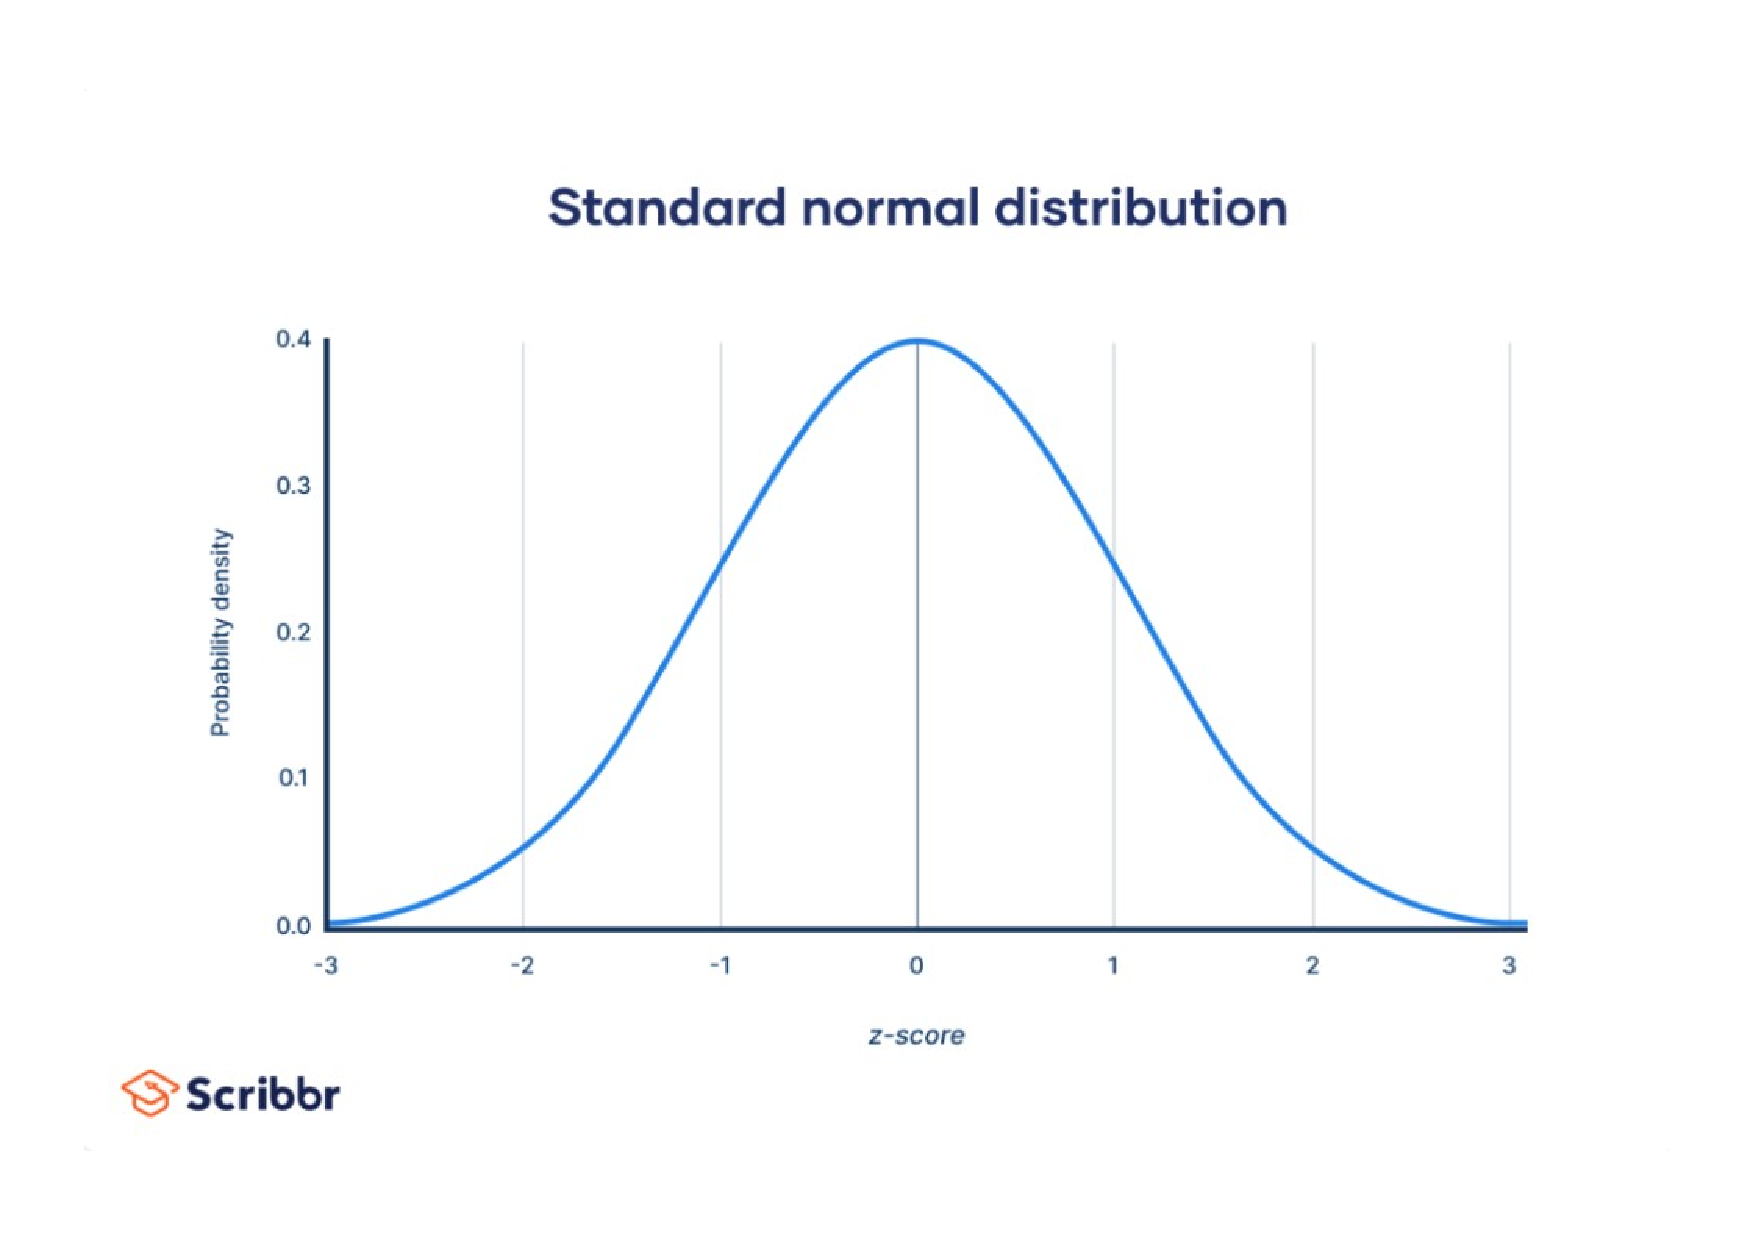
\includegraphics[width=0.6\linewidth]{figures/normal_distribution.pdf}
    \caption{The bell-shaped curve of the normal distribution}
    \label{fig:normal}
\end{figure}

The probability density function (PDF) of the normal distribution is defined as:

\begin{equation}
    \ f(x)= \cfrac{1}{\sigma\sqrt{2\pi}}\,exp\left({-\frac{(x-\mu)^2}{2\sigma^2}}\right)
\end{equation}

The symbol $\mu$ represents the mean, indicating the center of the data, while $\sigma$ is the standard deviation, describing the dispersion of the data. In the analysis of experimental data, understanding the normal distribution allows us to assess measurement errors, filter out outliers, and further build data models.

\subsubsection{Mean}
\hfill

The mean $\mu$ represents the central position of a dataset and serves as a typical value of the measurement results. When the same physical quantity is measured multiple times, the results may vary slightly each time, but they generally fluctuate around a certain value, which is the mean.
The mean can be calculated by dividing the sum of all data points by the total number of data points:
\begin{equation}
     \mu= \cfrac{1}{N}\sum_{i=1}^{N}x_i
\end{equation}

$x_i$ represents the ith measured value, and N is the number of measurements.
The mean helps us determine a representative value for a dataset, and in most cases, it can reflect the true value of the physical quantity.

% \clearpage

\subsubsection{Standard Deviation}
\hfill

The standard deviation $\sigma$ is used to measure the spread of data, indicating the degree of dispersion.

It is defined as:
\begin{equation}
     \sigma = \sqrt{\cfrac{1}{N}\sum_{i=1}^{N}{\left(x_i-\mu\right)^2}}
\end{equation}

\subsubsection{Standard Deviation Interval}
\hfill

In statistics, the so-called "68-95-99.7 rule" describes the application of standard deviation in data filtering:

\begin{enumerate}
    \item About 68\% of the data falls within $\pm$1 standard deviation of the mean.
    \item About 95\% of the data falls within $\pm$2 standard deviations of the mean.
    \item About 99.7\% of the data falls within $\pm$3 standard deviations of the mean.
\end{enumerate}
Therefore, if a data point significantly exceeds $\pm$3 standard deviations from the mean, it is highly likely to be an outlier.

\subsubsection{Data Filtering}
\hfill

In real-world physics experiments, the measurement process may be affected by environmental factors, equipment issues, or other sources of error, causing some data points to deviate from the normal range. To ensure accuracy in data analysis, data can be filtered based on standard deviation intervals.

In this experiment, we use Python to generate random data and determine whether each data point falls within $\pm$1 standard deviation of the mean, filtering out any anomalous values. This filtering method is widely applied in various scientific studies. For example, in astronomical observations, scientists need to remove anomalous data caused by atmospheric interference or other external factors.

\subsubsection{Data Visualization}
\hfill

We make the data more visually intuitive by creating charts, allowing us to observe the distribution of the data more clearly and identify trends or outliers. In this experiment, we use Matplotlib to plot a histogram to display the distribution of the data.

%%%%%%%%%%%%%%%%%
\clearpage
\section{Experimental steps}

\subsection{Practice 1}

\begin{figure}[h]
    \centering
    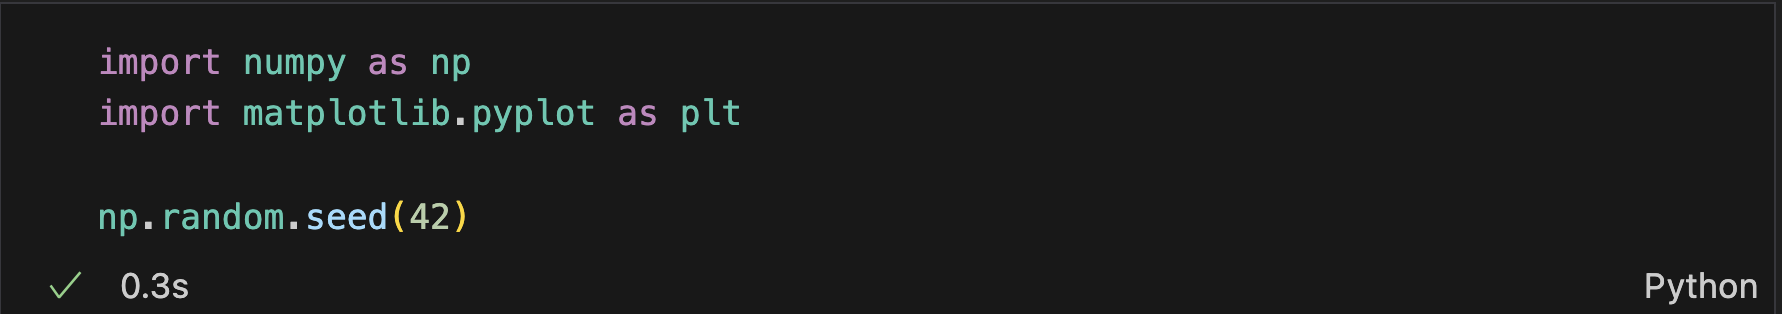
\includegraphics[width=0.9\linewidth]{figures/code/code_1_1.png}
    \caption{Import \texttt{numpy} and \texttt{matplotlib.pyplot} packages for better vectorized calculation and making plots. \texttt{np.random.seed(42)} is to keep the reproducibility.}
    \label{fig:code_1_1}
\end{figure}
\begin{enumerate}
    \item Generate a 1-d array with several elements, each element is sampled from a statistical population with a normal distribution with mean = 0 and standard deviation = 3.
    \begin{figure}[h]
        \centering
        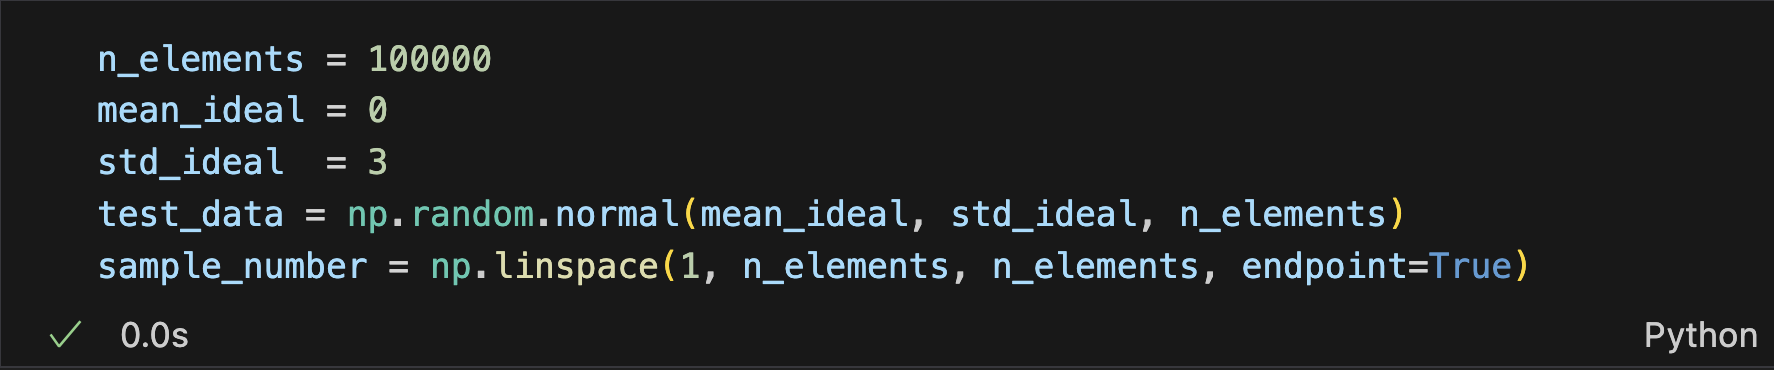
\includegraphics[width=0.9\linewidth]{figures/code/code_1_2.png}
        \caption{Initialize our samples (normal distribution of 10000 samples with mean = 0 and standard deviation = 3).}
        \label{fig:code_1_2}
    \end{figure}
    \item Plot the data points and mark the mean and standard deviation calculated from the data.
    \begin{figure}[h]
        \centering
        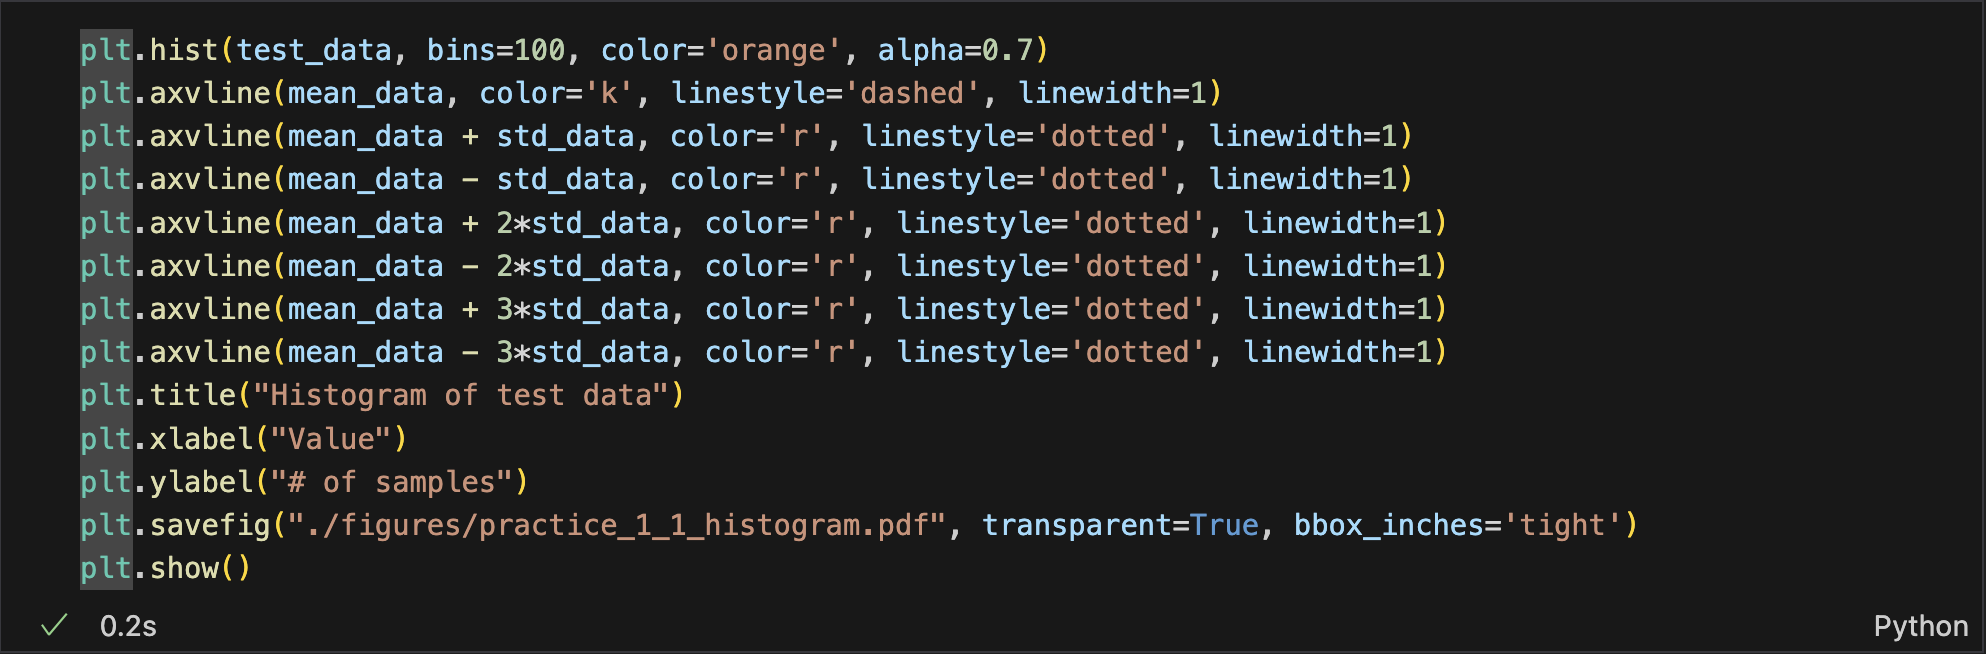
\includegraphics[width=0.9\linewidth]{figures/code/code_1_4.png}
        \caption{Code for making histogram of our samples}
        \label{fig:code_1_4}
    \end{figure}
    \clearpage
    \begin{figure}[h]
        \centering
        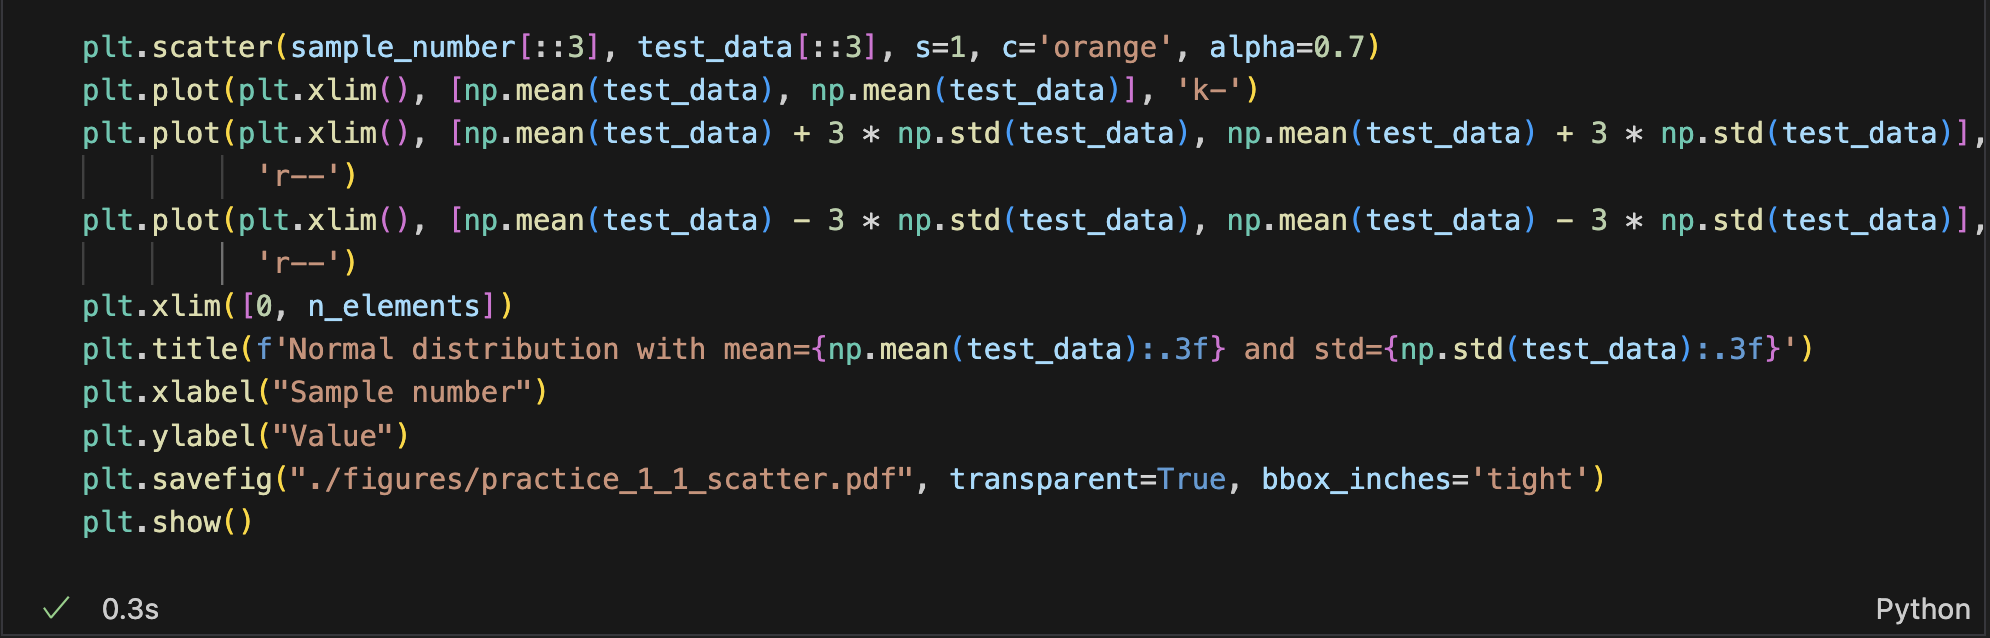
\includegraphics[width=0.9\linewidth]{figures/code/code_1_5.png}
        \caption{Code for making scattered plot of our samples}
        \label{fig:code_1_5}
    \end{figure}

    \item Will the mean and standard deviation be the same as the population?\\
\end{enumerate}

\subsection{Practice 2}

\begin{figure}[h]
    \centering
    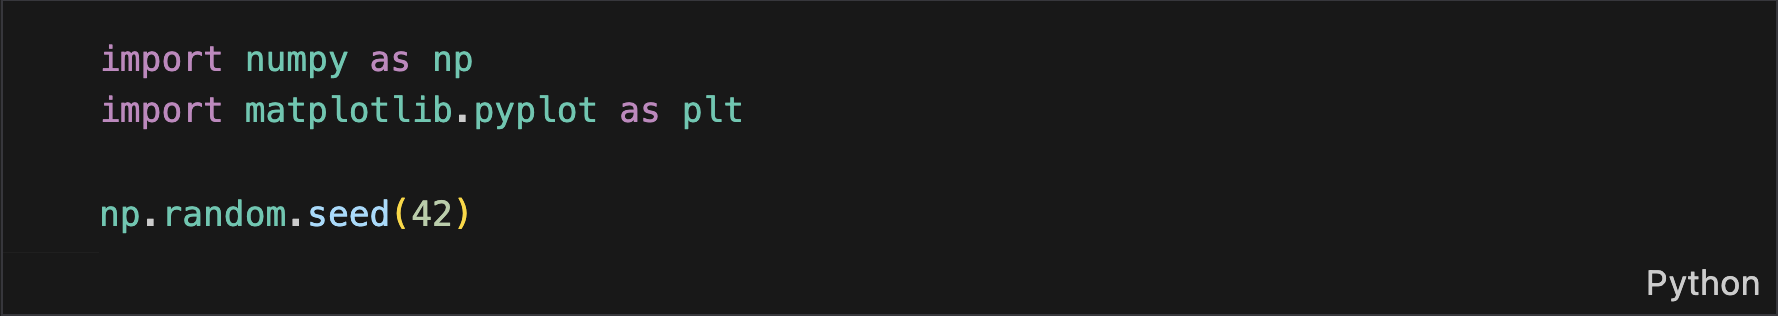
\includegraphics[width=0.9\linewidth]{figures/code/code_2_1.png}
    \caption{Import \texttt{numpy} and \texttt{matplotlib.pyplot} packages for better vectorized calculation and making plots}
    \label{fig:code_2_1}
\end{figure}

\begin{enumerate}
    \item Generate a 1-d array with 50 elements, each element is sampled from a statistical population with a normal distribution with mean = 0 and standard deviation = 3.
    \begin{figure}[h]
        \centering
        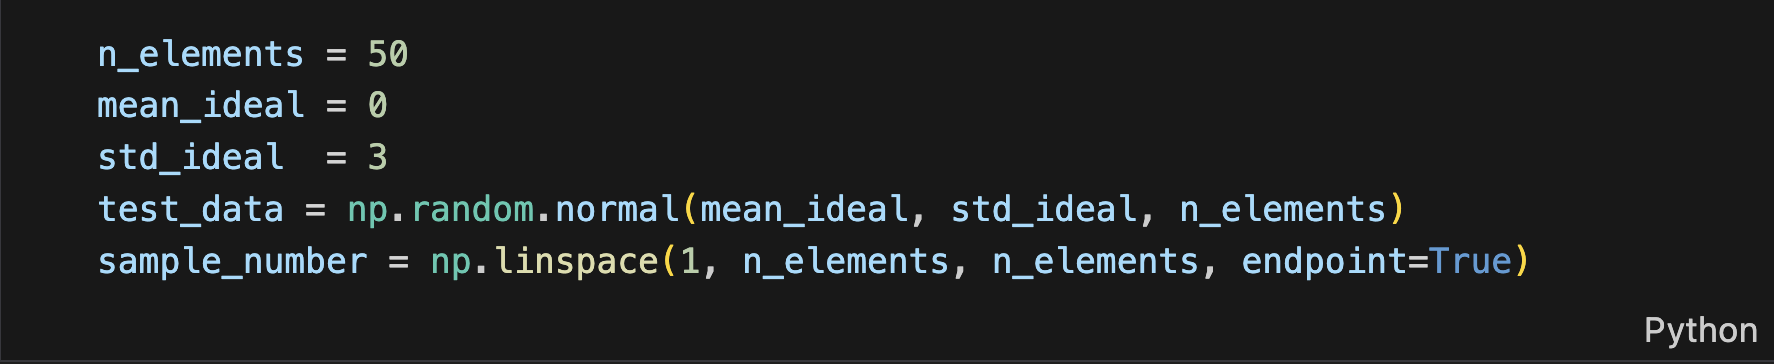
\includegraphics[width=0.9\linewidth]{figures/code/code_2_2.png}
        \caption{Initialize our samples (normal distribution of 50 samples with mean = 0 and standard deviation = 3).}
        \label{fig:code_2_2}
    \end{figure}
    \clearpage
    \begin{figure}[h]
        \centering
        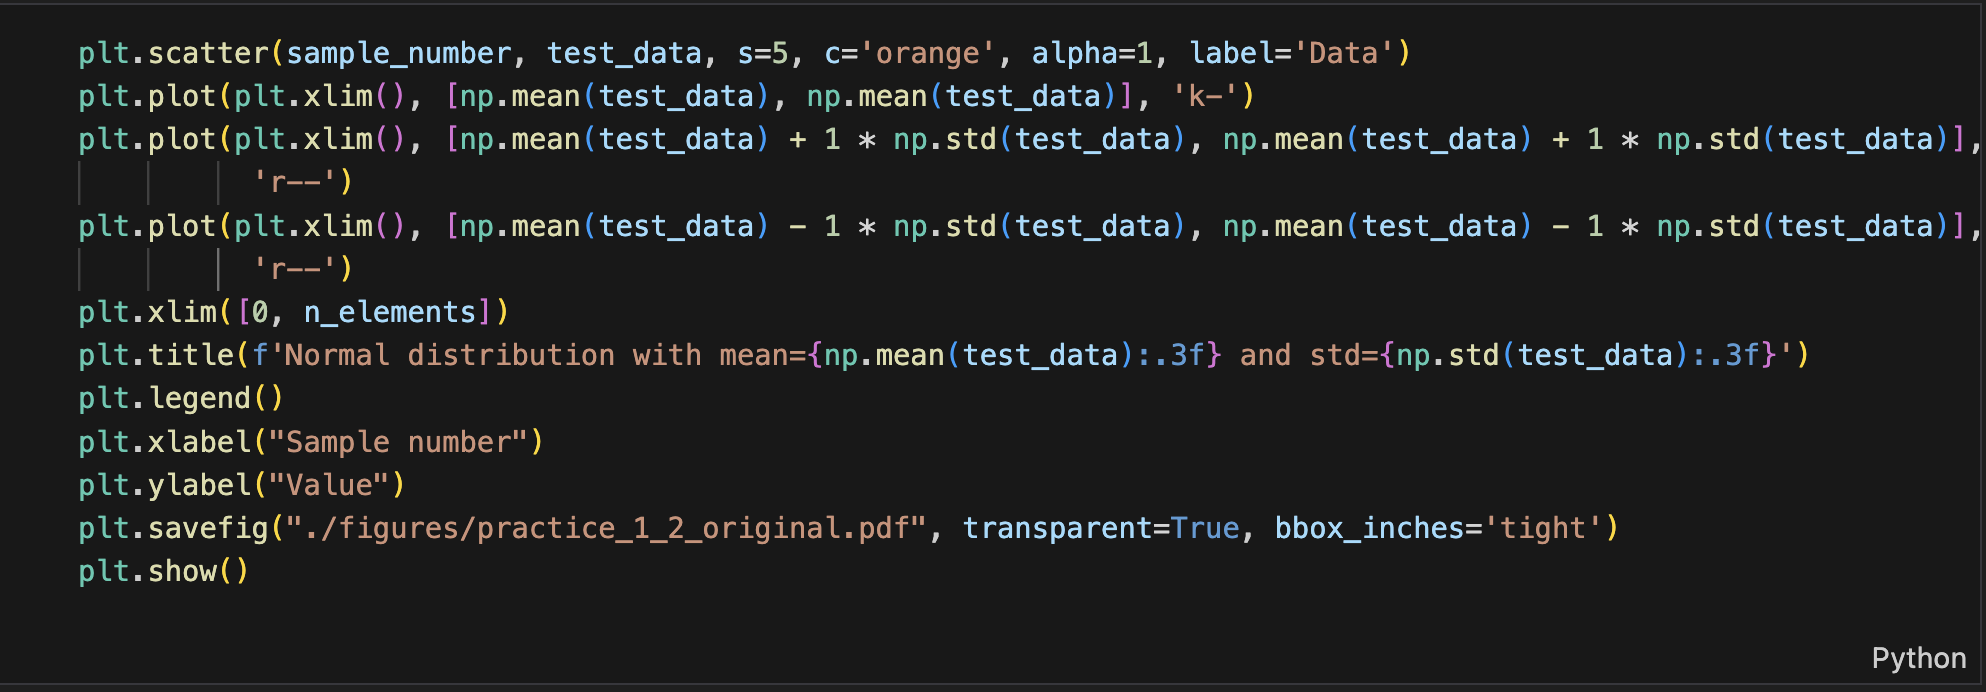
\includegraphics[width=0.9\linewidth]{figures/code/code_2_4.png}
        \caption{Code for making scattered plot of our samples}
        \label{fig:code_2_4}
    \end{figure}
    \item Pick up the data points that are within 1 standard deviation from the mean.
    \begin{figure}[h]
        \centering
        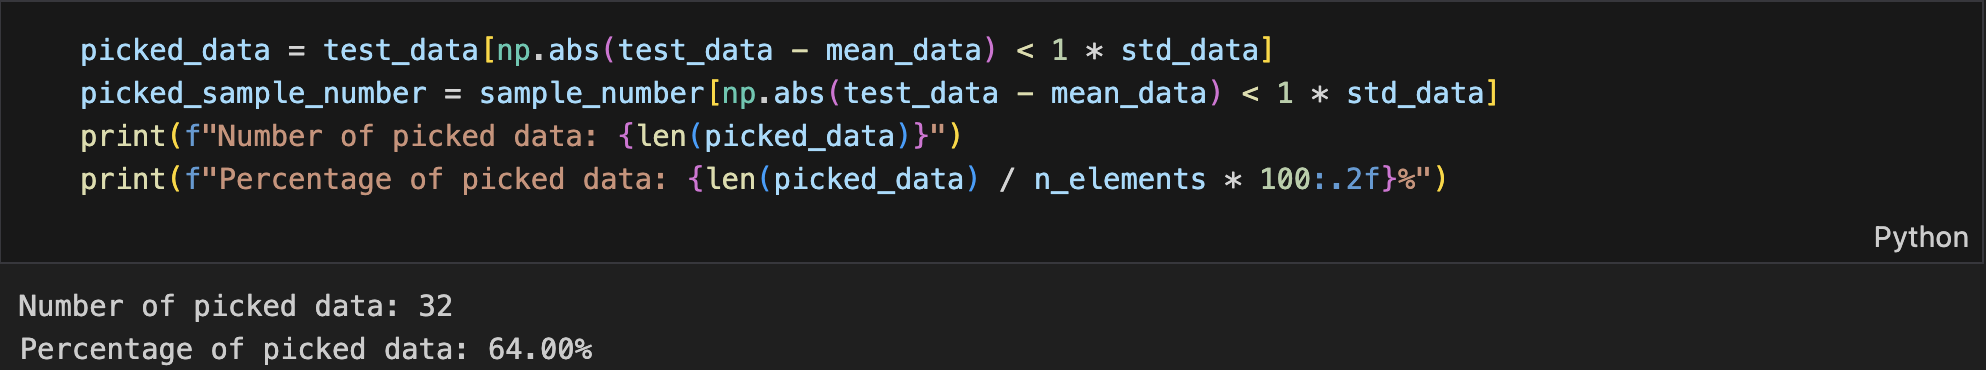
\includegraphics[width=0.9\linewidth]{figures/code/code_2_5.png}
        \caption{Total number of picked data is 32 and the percentage of picked data is 64\%}
        \label{fig:code_2_5}
    \end{figure}
    \item Plot the picked data points and original data points to check if the filtering process is correct.
    \item Mark the $mean-stdev$ and $mean+stdev$ on the plot might be helpful.
    \begin{figure}[h]
        \centering
        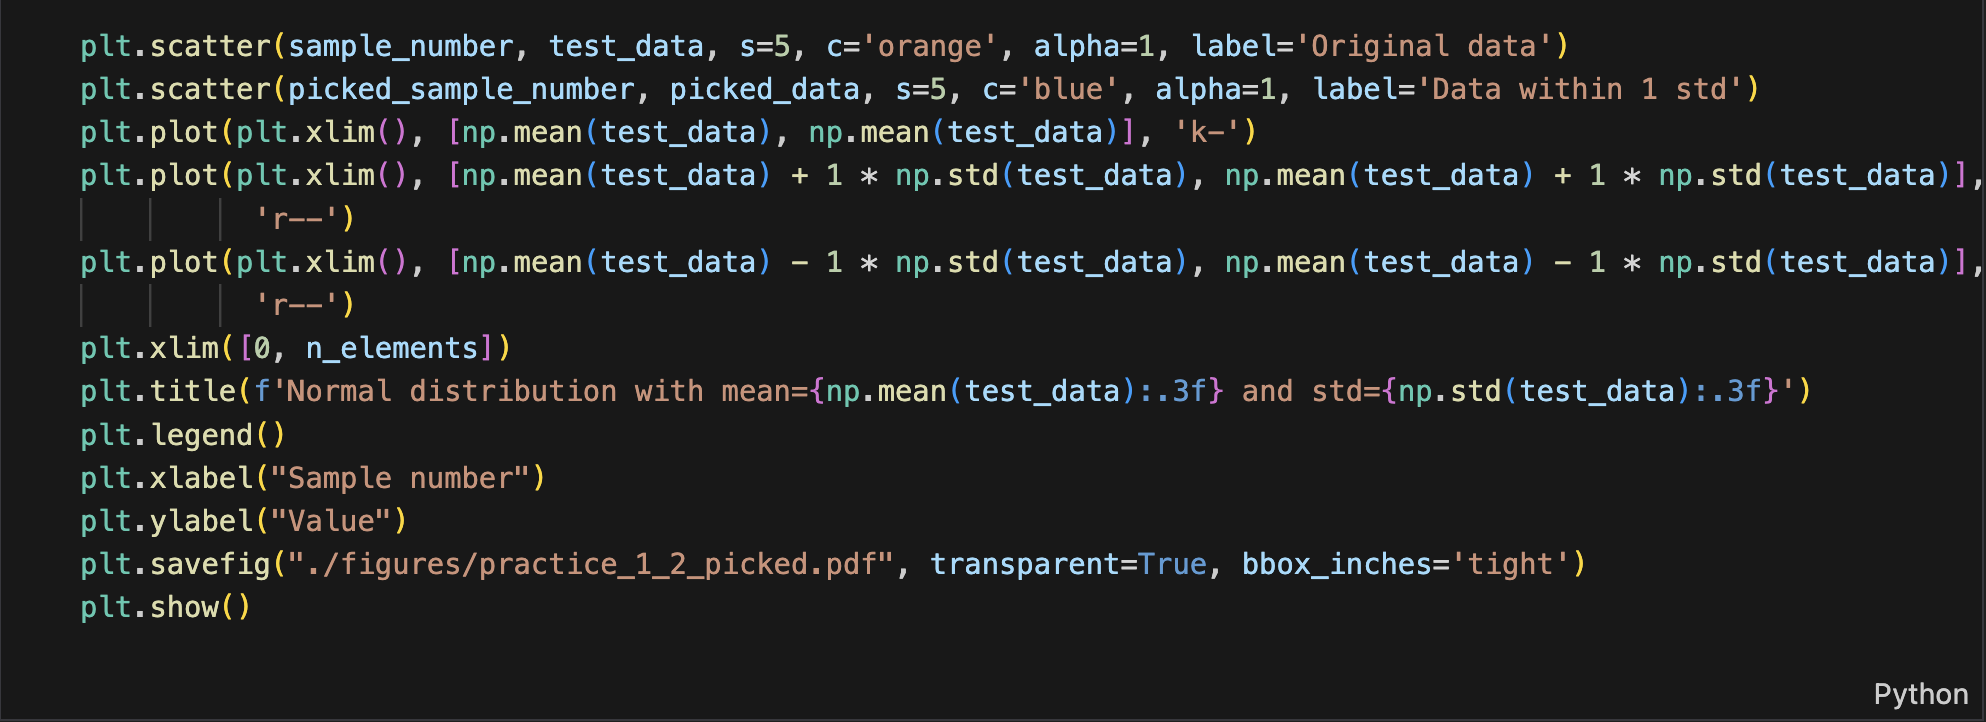
\includegraphics[width=0.9\linewidth]{figures/code/code_2_6.png}
        \caption{Code for making scattered plot of our samples}
        \label{fig:code_2_6}
    \end{figure}
    \item Print all the indices of the data points that are picked (These indices might range from 0 to 49).
\end{enumerate}


\clearpage
\subsection{Practice 3}

\begin{figure}[h]
    \centering
    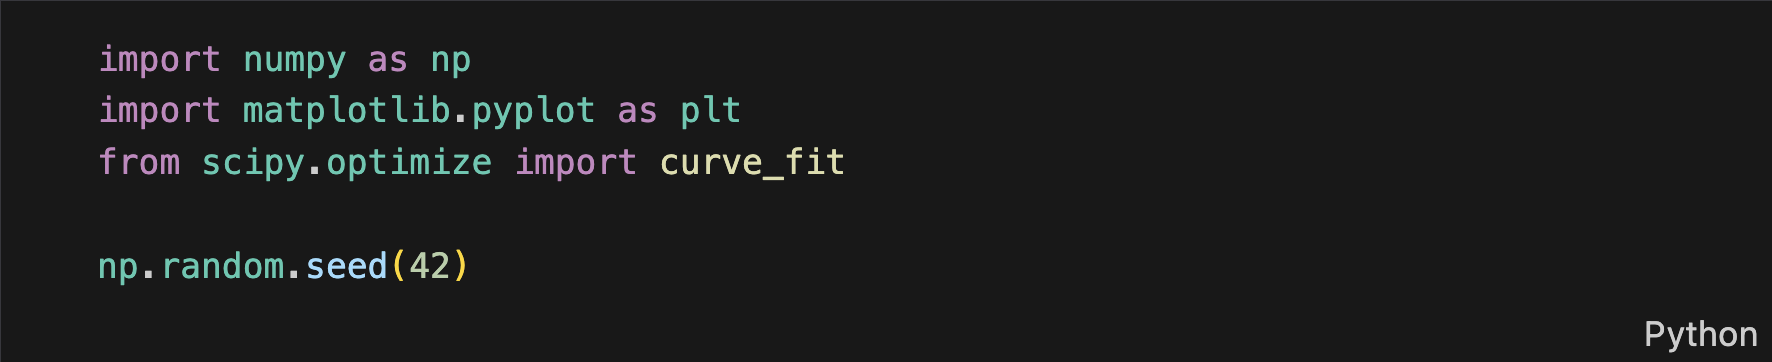
\includegraphics[width=0.9\linewidth]{figures/code/code_3_1.png}
    \caption{Import \texttt{numpy} and \texttt{matplotlib.pyplot} packages for better vectorized calculation and making plots. Also, from \texttt{scipy.optimize} package to import \texttt{curve\_fit} function for fitting}
    \label{fig:code_3_1}
\end{figure}

\begin{figure}[h]
    \centering
    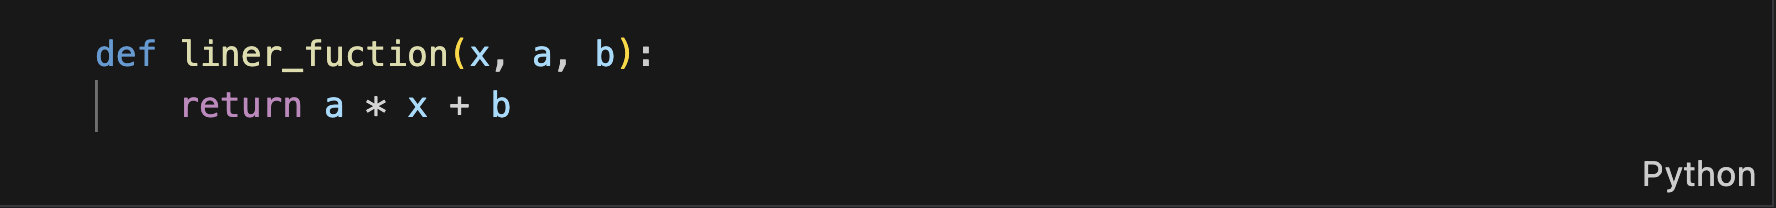
\includegraphics[width=0.9\linewidth]{figures/code/code_3_2.png}
    \caption{Define a liner function $y =a*x +b$.}
    \label{fig:code_3_2}
\end{figure}
\begin{enumerate}
    \item Generate a set of data points defined by a function $y =a*x +b +noise$ with \texttt{x = np.linspace(1, 10, 10)}.
    \item The noise is sampled from a normal distribution with mean = 0 and standard deviation = $\sigma_0$. (define $\sigma_0$ whatever you like)
    \begin{figure}[h]
        \centering
        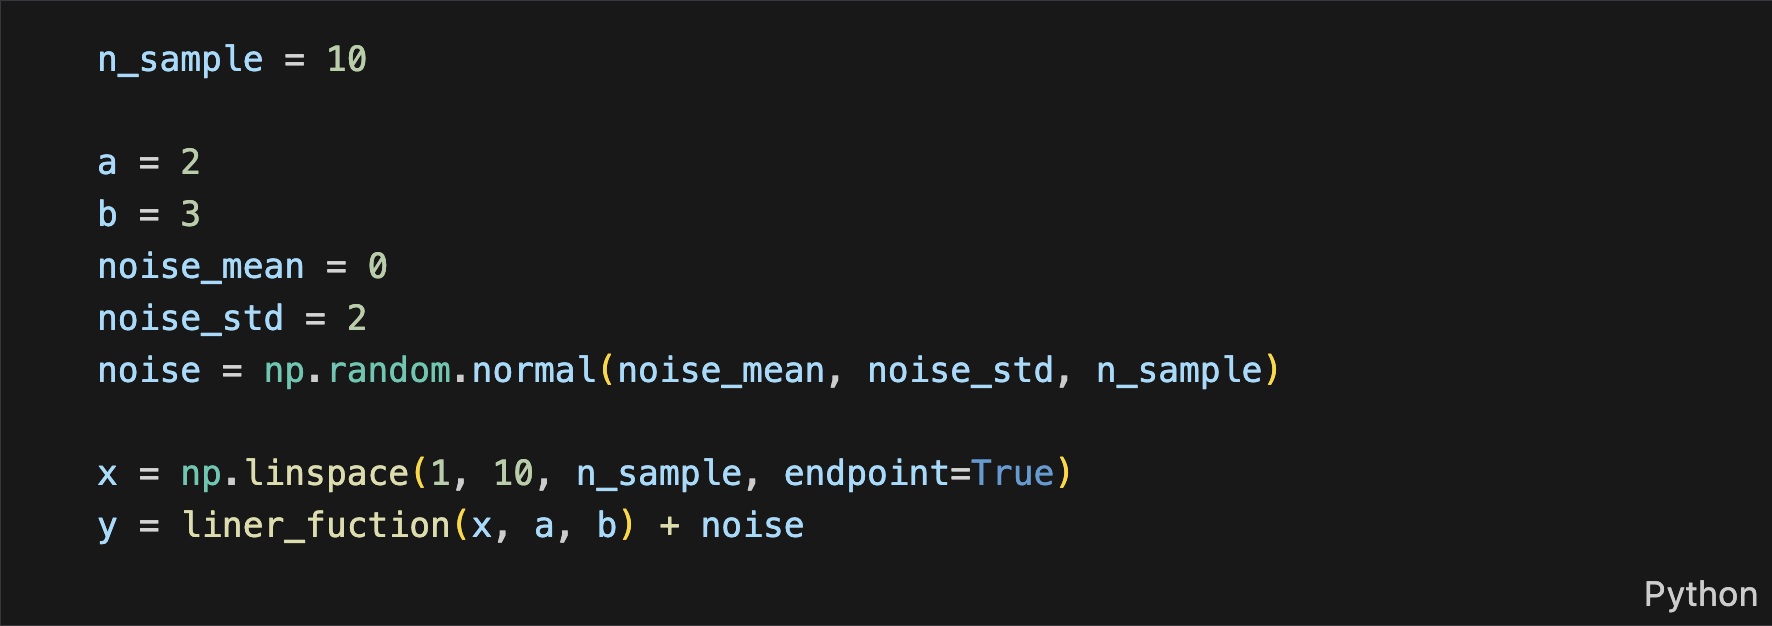
\includegraphics[width=0.9\linewidth]{figures/code/code_3_3.png}
        \caption{Initialize $x$ (\texttt{np.linspace(1, 10, 10)}) and $y =a*x +b +noise$ where the noise is the normal distribution with mean =0 and standard deviation = 2}
        \label{fig:code_3_3}
    \end{figure}
    % \clearpage
    \item Use the \texttt{curve\_fit} function in \texttt{scipy.optimize} to fit the data points with the function $y =a*x +b$.
    \begin{figure}[h]
        \centering
        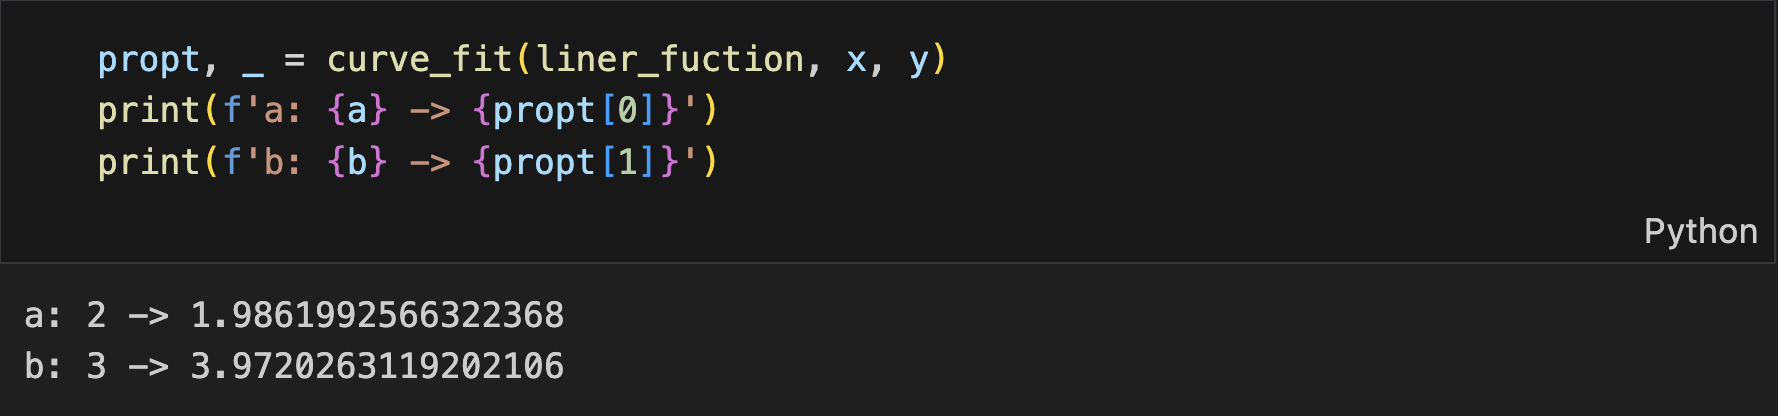
\includegraphics[width=0.9\linewidth]{figures/code/code_3_5.png}
        \caption{Fit the noisy $y$ with the linear function (Fig.\ref{fig:code_3_2}) with \texttt{curve\_fit}.}
        \label{fig:code_3_5}
    \end{figure}
    \item Plot the data points and the fitting curve.
    \begin{figure}[h]
        \centering
        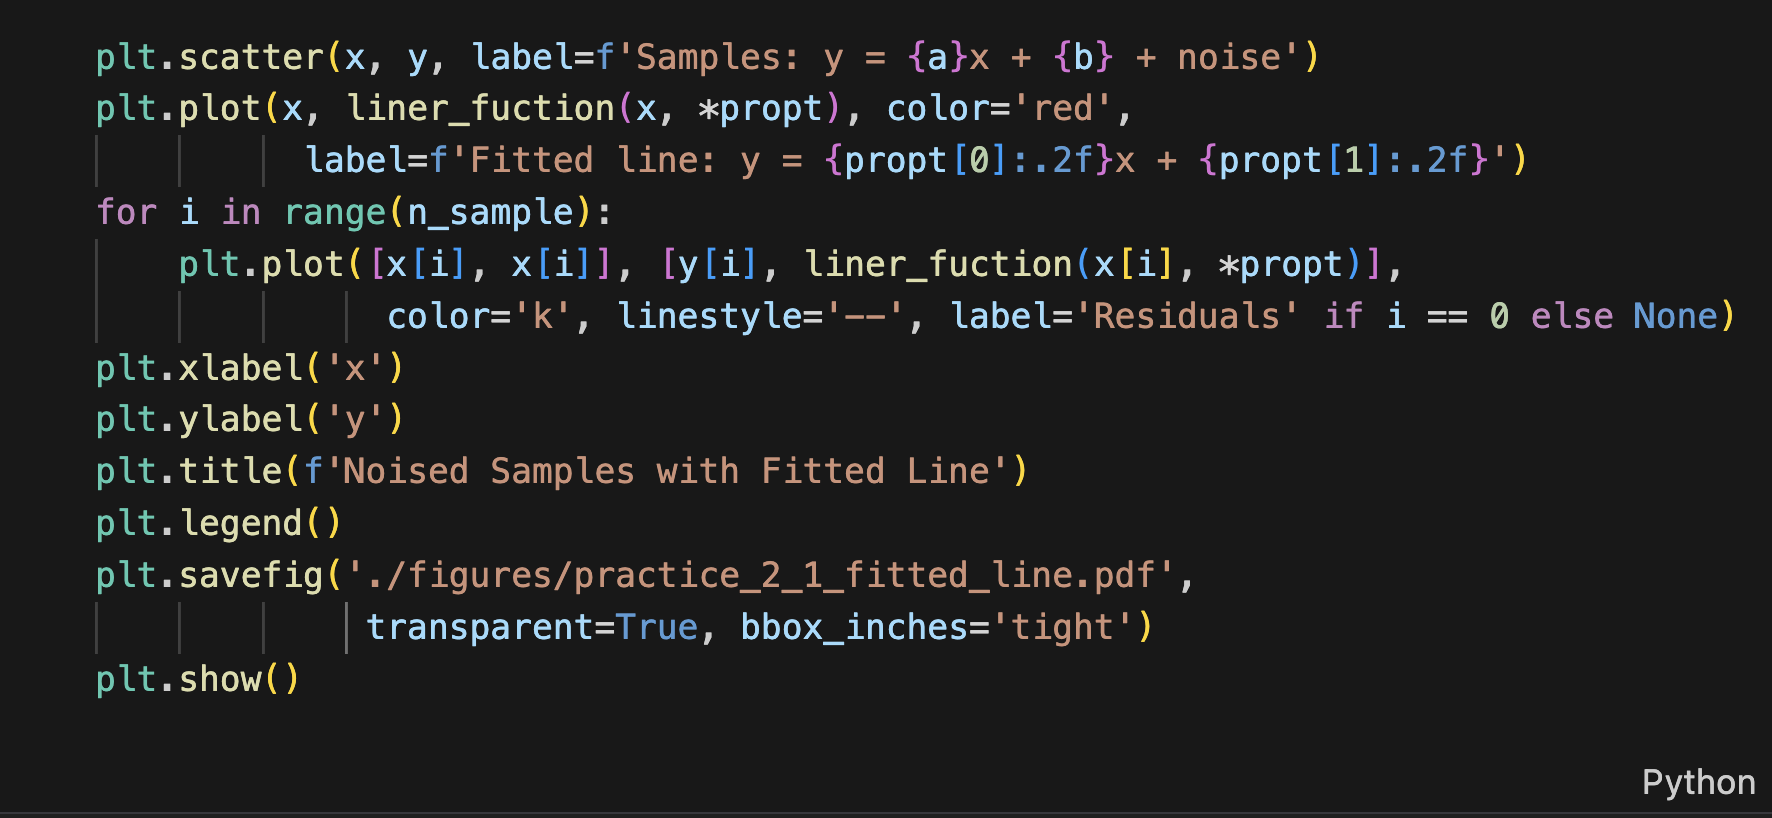
\includegraphics[width=0.9\linewidth]{figures/code/code_3_6.png}
        \caption{Code to plot the data points and the fitting curve}
        \label{fig:code_3_6}
    \end{figure}
    % \clearpage
    \item Calculate the residuals and plot the residuals.
    \begin{figure}[h]
        \centering
        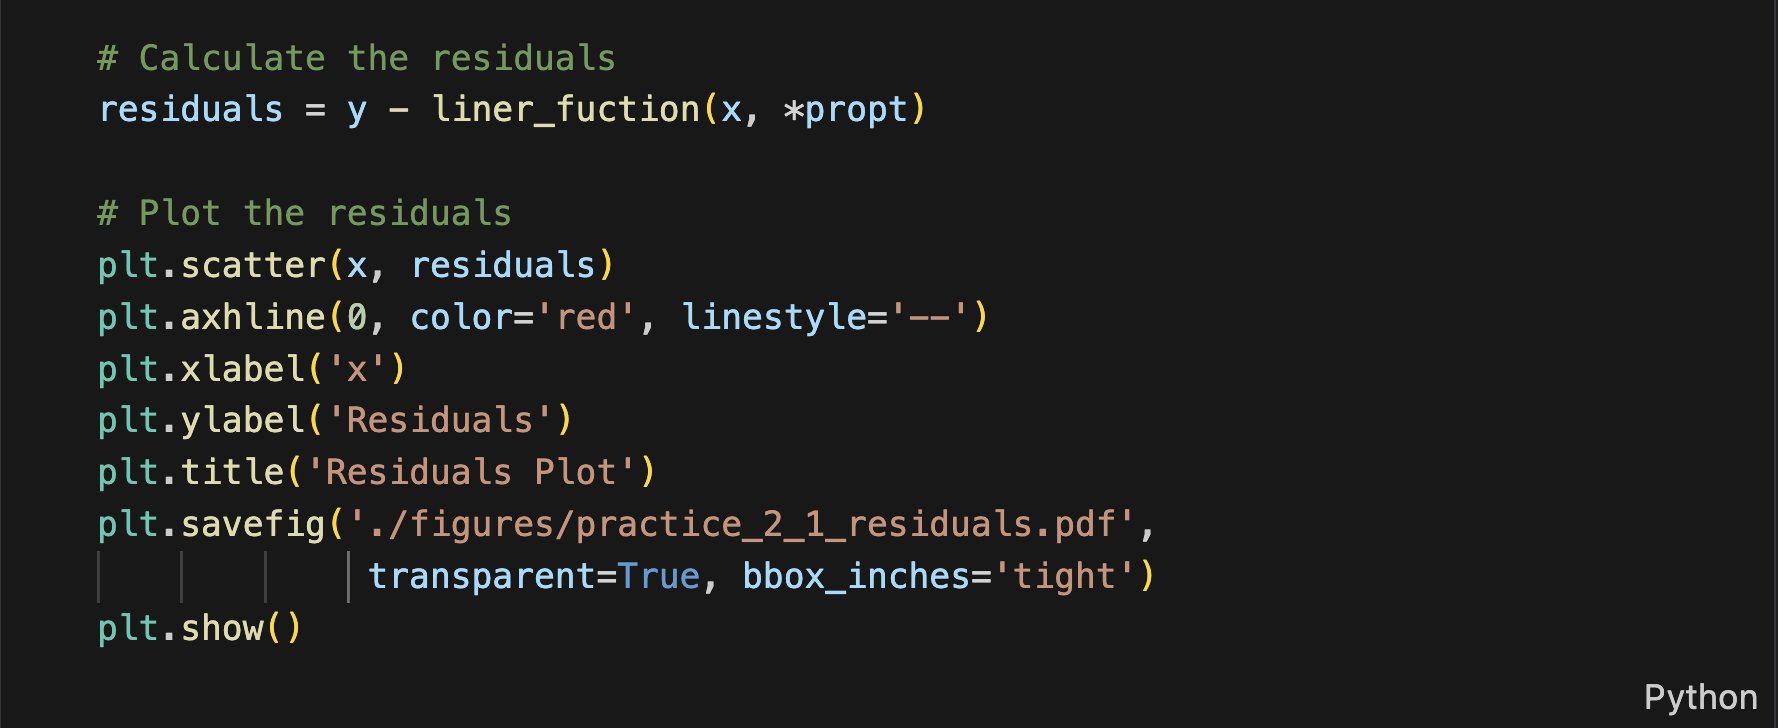
\includegraphics[width=0.9\linewidth]{figures/code/code_3_7.png}
        \caption{Code to plot the residuals.}
        \label{fig:code_3_7}
    \end{figure}
\end{enumerate}

\clearpage
\subsection{Practice 4}

\begin{figure}[h]
    \centering
    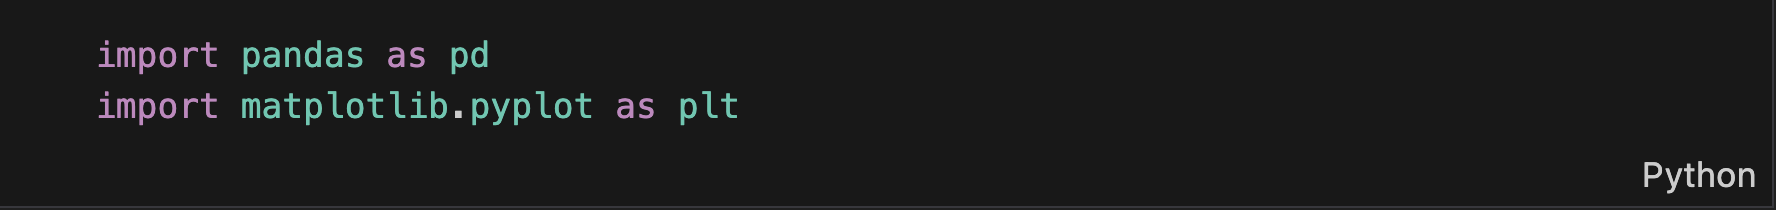
\includegraphics[width=0.9\linewidth]{figures/code/code_4_1.png}
    \caption{Import \texttt{panda} and \texttt{matplotlib.pyplot} packages to read csv files and make plots, respectively}
    \label{fig:code_4_1}
\end{figure}
\begin{enumerate}
    \item Read out the data from a csv file.
    \item Plot the data points.
    \item The following is an example of how to read out the data from a csv file.
    \item You can modify the code to read out the data from the file you have
\end{enumerate}

% \begin{figure}[h]
%     \centering
%     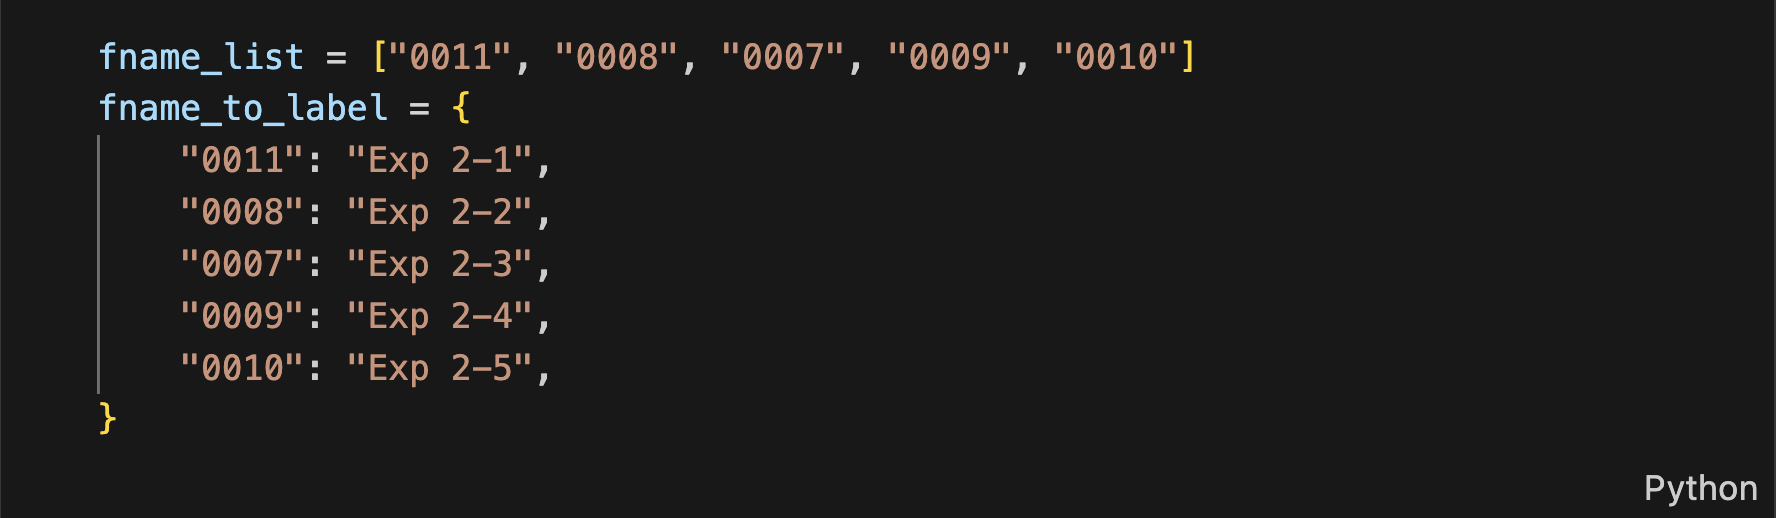
\includegraphics[height=3cm]{figures/code/code_4_2.png}
%     \caption{File names to be read.}
%     \label{fig:code_4_2}
% \end{figure}

\begin{figure}[h]
    \centering
    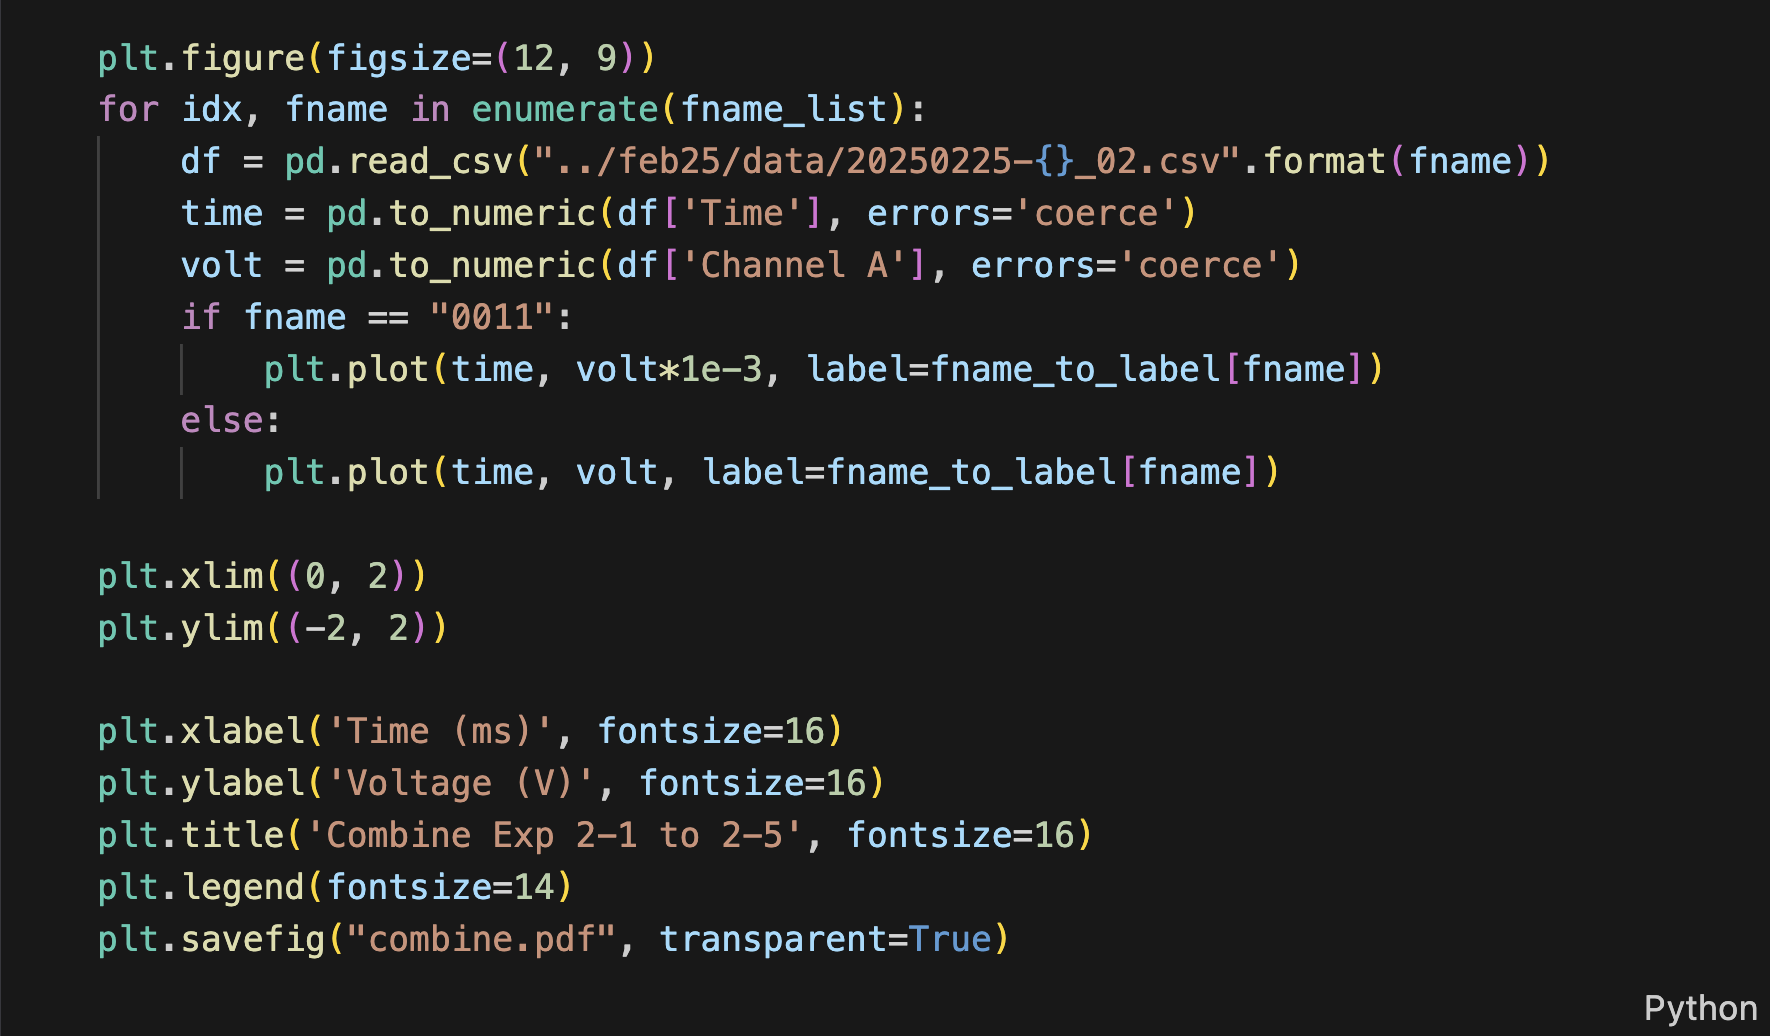
\includegraphics[width=0.9\linewidth]{figures/code/code_4_3.png}
    \caption{Using "for loop" to iteratively read files and plot the data.}
    \label{fig:code_4_3}
\end{figure}


\clearpage
\section{Result}\label{sec:result}

\subsection{Practice 1}

\begin{figure}[h]
    \centering
    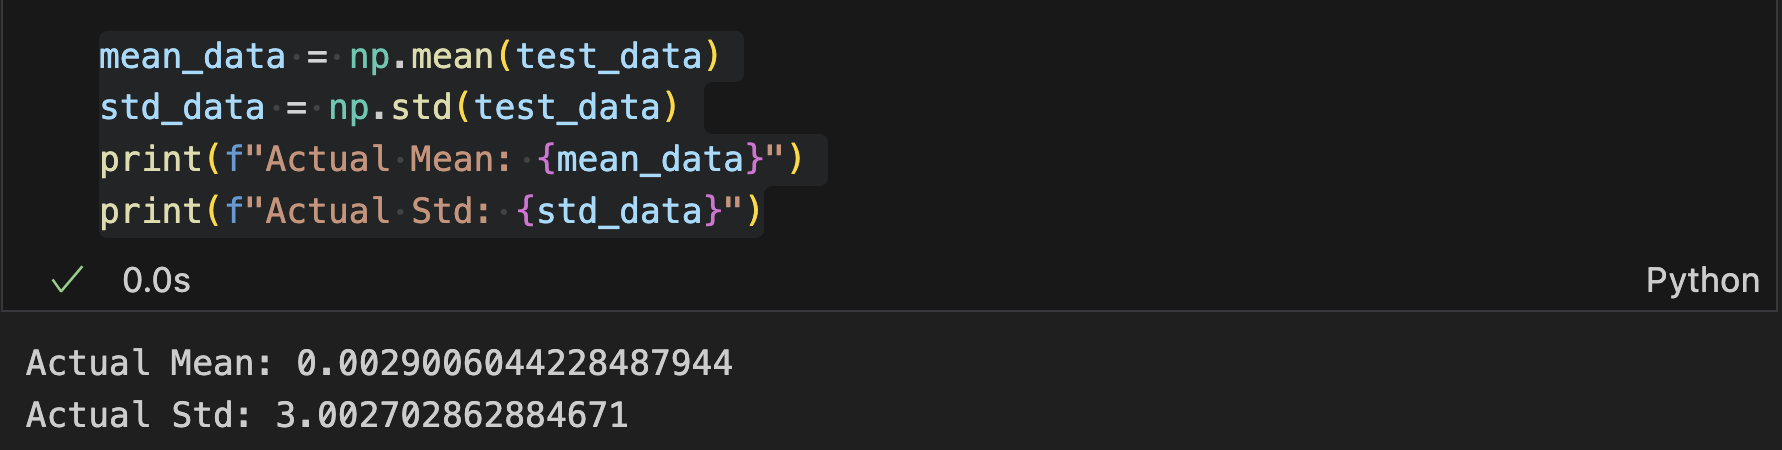
\includegraphics[width=0.9\linewidth]{figures/code/code_1_3.png}
    \caption{The actual mean $\mu$ and standard deviation $\sigma$ of our sample: $\mu \approx 0.0029$, $\sigma \approx 3.0027$}
    \label{fig:actual_1_3}
\end{figure}
\begin{figure}[h]
    \centering
    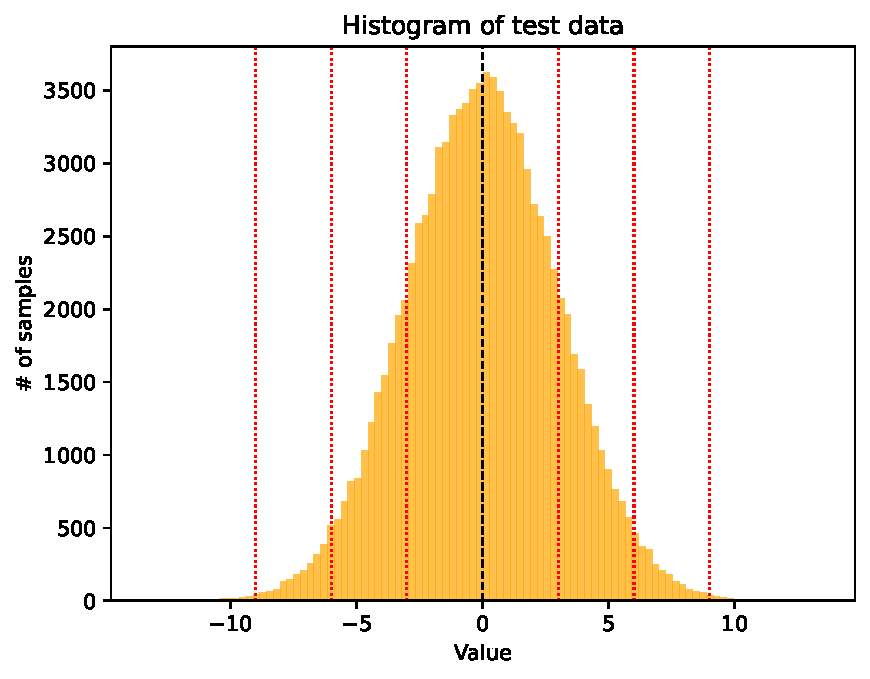
\includegraphics[width=0.45\linewidth]{figures/practice_1_1_histogram.pdf}
    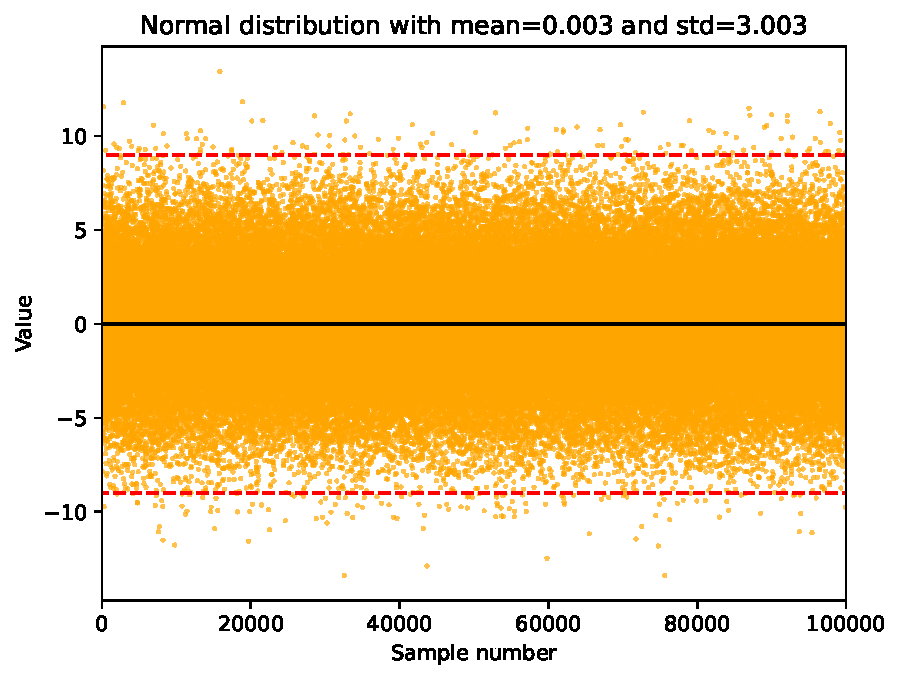
\includegraphics[width=0.45\linewidth]{figures/practice_1_1_scatter.pdf}
    \caption{\textit{left}: The distribution of our samples (normal distribution of 10000 samples with mean = 0 and standard deviation = 3). The black dashed line labels the mean of the samples, and the red dotted lines from inner to outer represent the range of $\pm 1\sigma$, $\pm 2\sigma$, and $\pm 3\sigma$, respectively. \textit{right}: The data points of our samples. The black solid line labels the mean of the samples, and the red dashed lines note the range with $\pm 3\sigma$.}
    \label{fig:practice_1}
\end{figure}
% \begin{figure}[h]
%     \centering
%     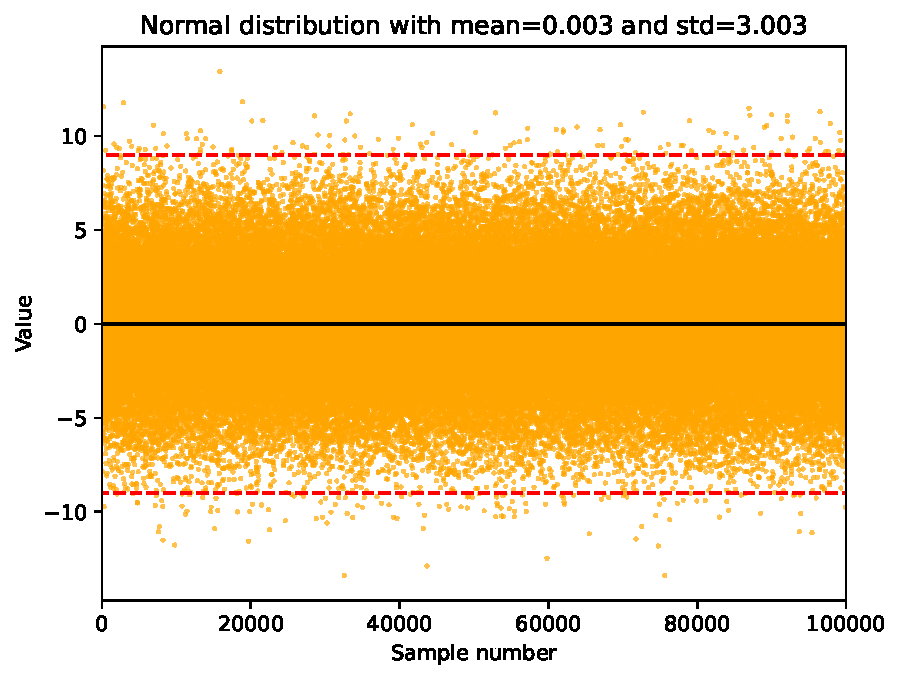
\includegraphics[width=0.49\linewidth]{figures/practice_1_1_scatter.pdf}
%     \caption{The data points of our samples. The black solid line labels the mean of the samples, and the red dashed lines note the range with $\pm 3\sigma$.}
%     \label{fig:practice_2}
% \end{figure}

\clearpage
\subsection{Practice 2}

\begin{figure}[h]
    \centering
    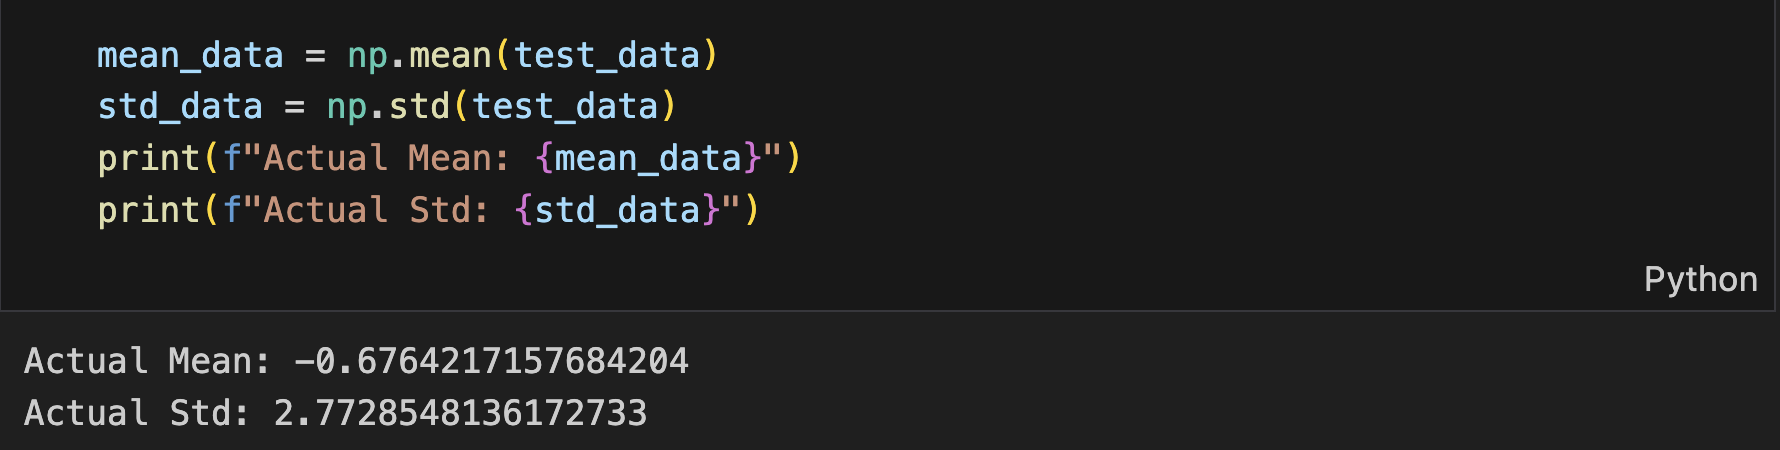
\includegraphics[width=0.8\linewidth]{figures/code/code_2_3.png}
    \caption{The actual mean $\mu$ and standard deviation $\sigma$ of our sample: $\mu \approx -0.6764$, $\sigma \approx 2.7729$}
    \label{fig:code_2_3}
\end{figure}
\begin{figure}[h]
    \centering
    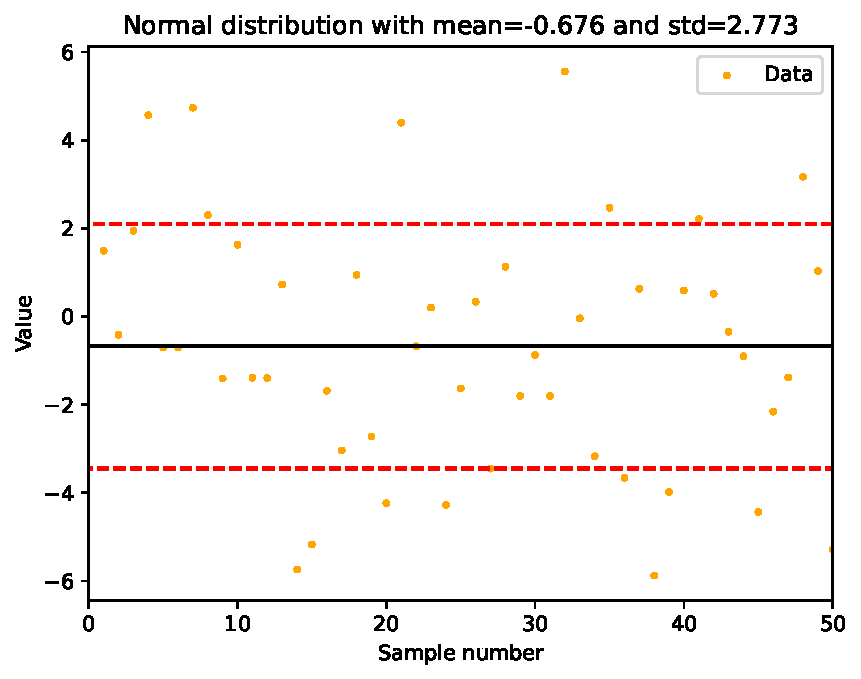
\includegraphics[width=0.45\linewidth]{figures/practice_1_2_original.pdf}
    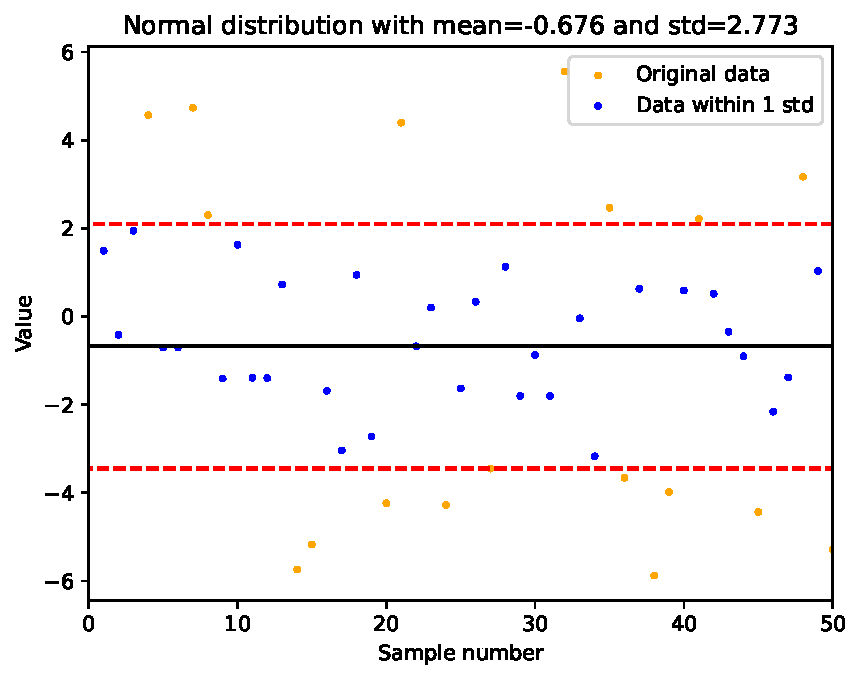
\includegraphics[width=0.45\linewidth]{figures/practice_1_2_picked.pdf}
    \caption{\textit{left}: The data points of our samples (normal distribution of 50 samples with mean = 0 and standard deviation = 3). The black solid line labels the mean of the samples, and the red dashed lines note the range with $\pm 1\sigma$. \textit{right}: The same plot but the blue points are within $\pm 1\sigma$.}
    \label{fig:practice_2_1}
\end{figure}

% \begin{figure}[h]
%     \centering
%     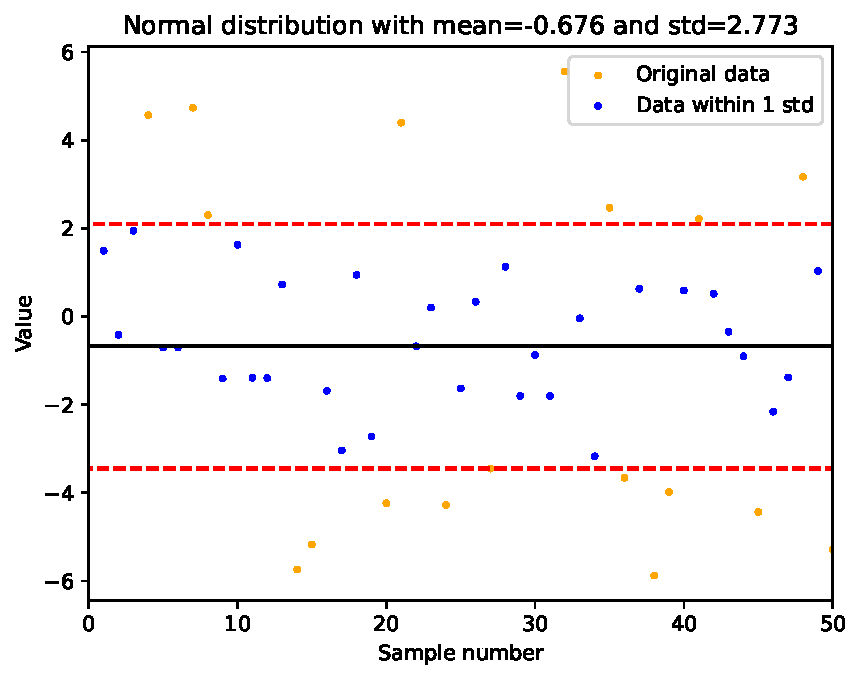
\includegraphics[width=0.9\linewidth]{figures/practice_1_2_picked.pdf}
%     \caption{The same plot as Fig.\ref{fig:practice_2_1} but the orange points are the data outside the $\pm 1\sigma$, and the blue points are within $\pm 1\sigma$.}
%     \label{fig:practice_2_2}
% \end{figure}
\begin{figure}[h]
    \centering
    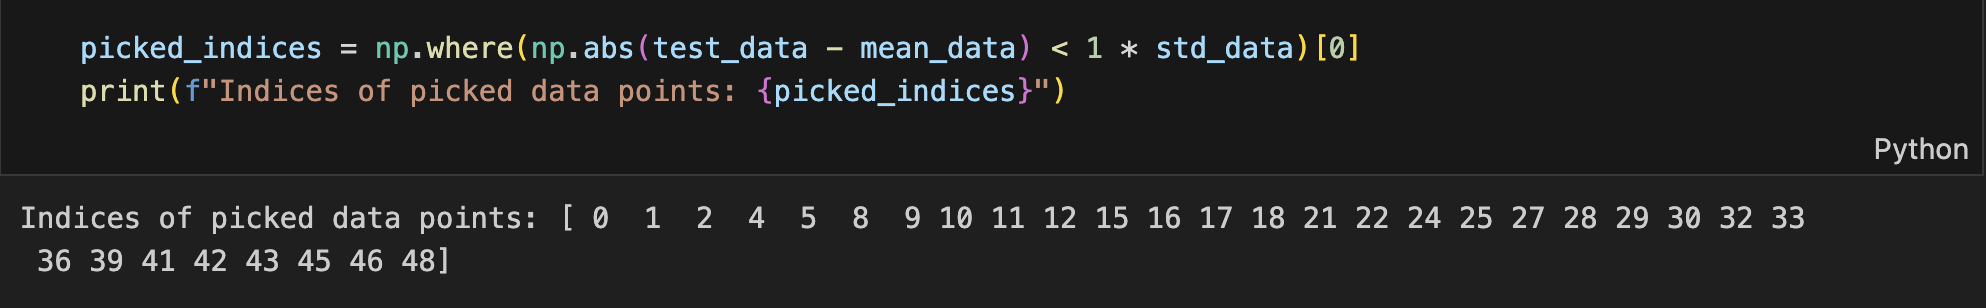
\includegraphics[width=0.8\linewidth]{figures/code/code_2_7.png}
    \caption{Print all the indices of the data points that are picked (The indices of the data points that are picked: 0, 1, 2, 4, 5, 8, 9, 10, 11, 12, 15, 16, 17, 18, 21, 22, 24, 25, 27, 28, 29, 30, 32, 33, 36, 39, 41, 42, 43, 45, 46, 48)}
    \label{fig:code_2_7}
\end{figure}

\clearpage
\subsection{Practice 3}

\begin{figure}[h]
    \centering
    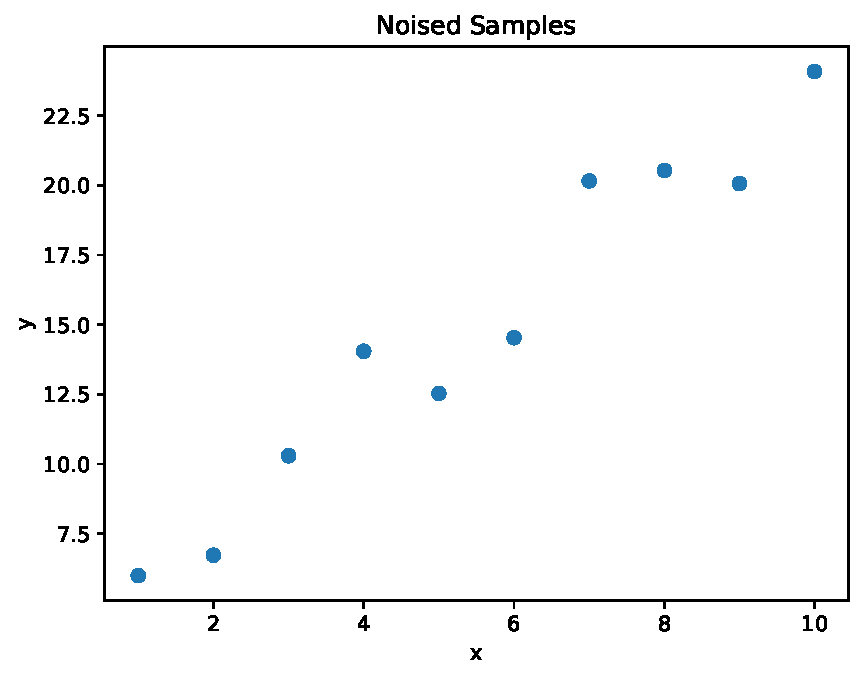
\includegraphics[width=0.45\linewidth]{figures/practice_2_1_original_samples.pdf}
    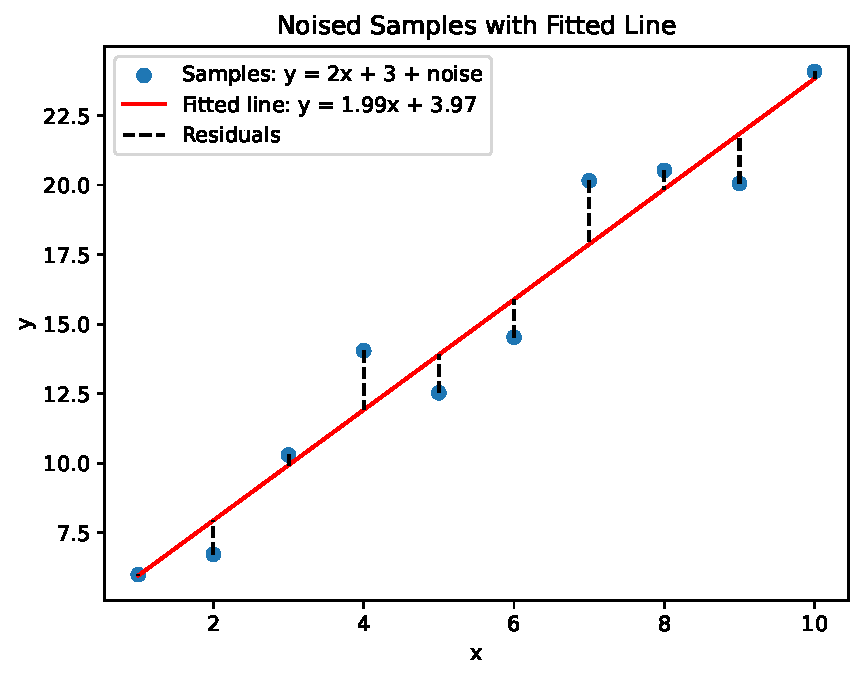
\includegraphics[width=0.45\linewidth]{figures/practice_2_1_fitted_line.pdf}
    \caption{\textit{left}: The scattered plot of of $x$ (\texttt{np.linspace(1, 10, 10)}) and $y =a*x +b +noise$ where the noise is the normal distribution with mean =0 and standard deviation = 2. \textit{right}: The data point $(x, y)$ (blue dots) and the fitted curve $(x, y_{fit})$ (red line). The residuals of each point are also labeled with black dashed lines on blue dots.}
    \label{fig:practice_2_1_original}
\end{figure}
% \begin{figure}[h]
%     \centering
%     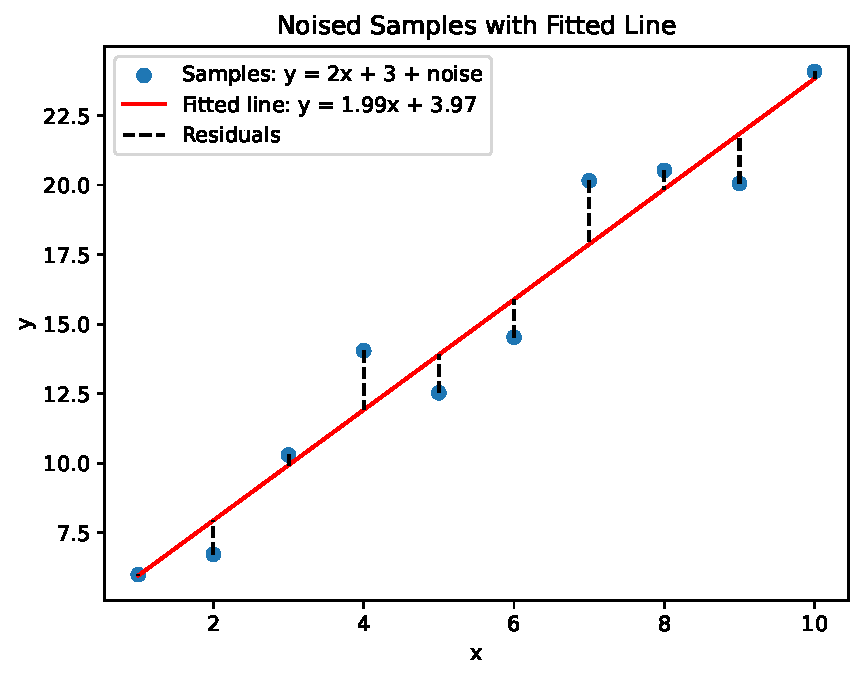
\includegraphics[width=0.9\linewidth]{figures/practice_2_1_fitted_line.pdf}
%     \caption{The data point $(x, y)$ (blue dots) and the fitted curve $(x, y_{fit})$ (red line). The residuals of each point are also labeled with black dashed lines on blue dots.}
%     \label{fig:practice_2_1_fit}
% \end{figure}
\begin{figure}[h]
    \centering
    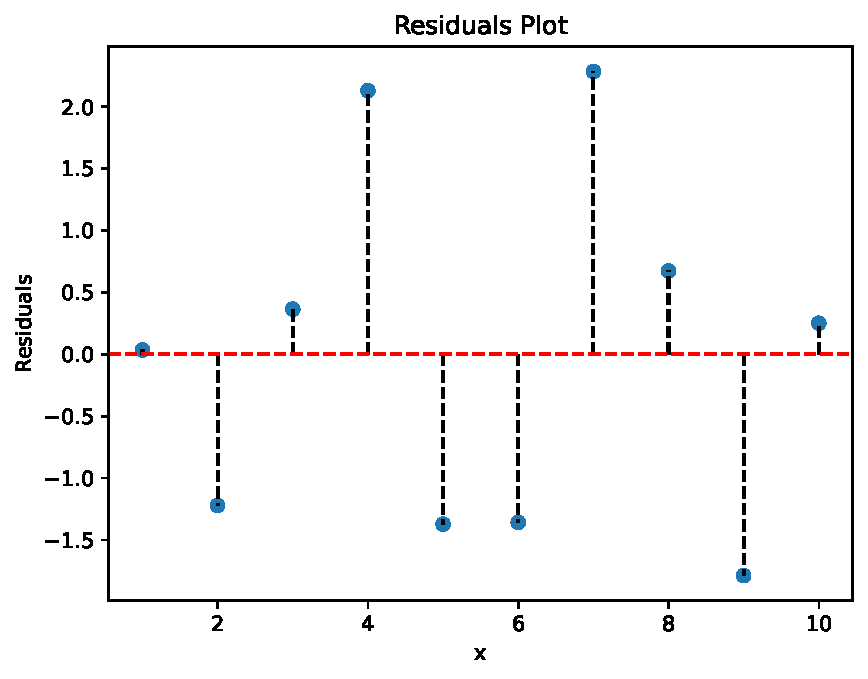
\includegraphics[width=0.65\linewidth]{figures/practice_2_1_residuals.pdf}
    \caption{The extracted residuals from Fig.\ref{fig:practice_2_1_original}. The horizontal red line labels residual=0}
    \label{fig:practice_2_1_residual}
\end{figure}

\clearpage
\subsection{Practice 4}

\begin{figure}[h]
    \centering
    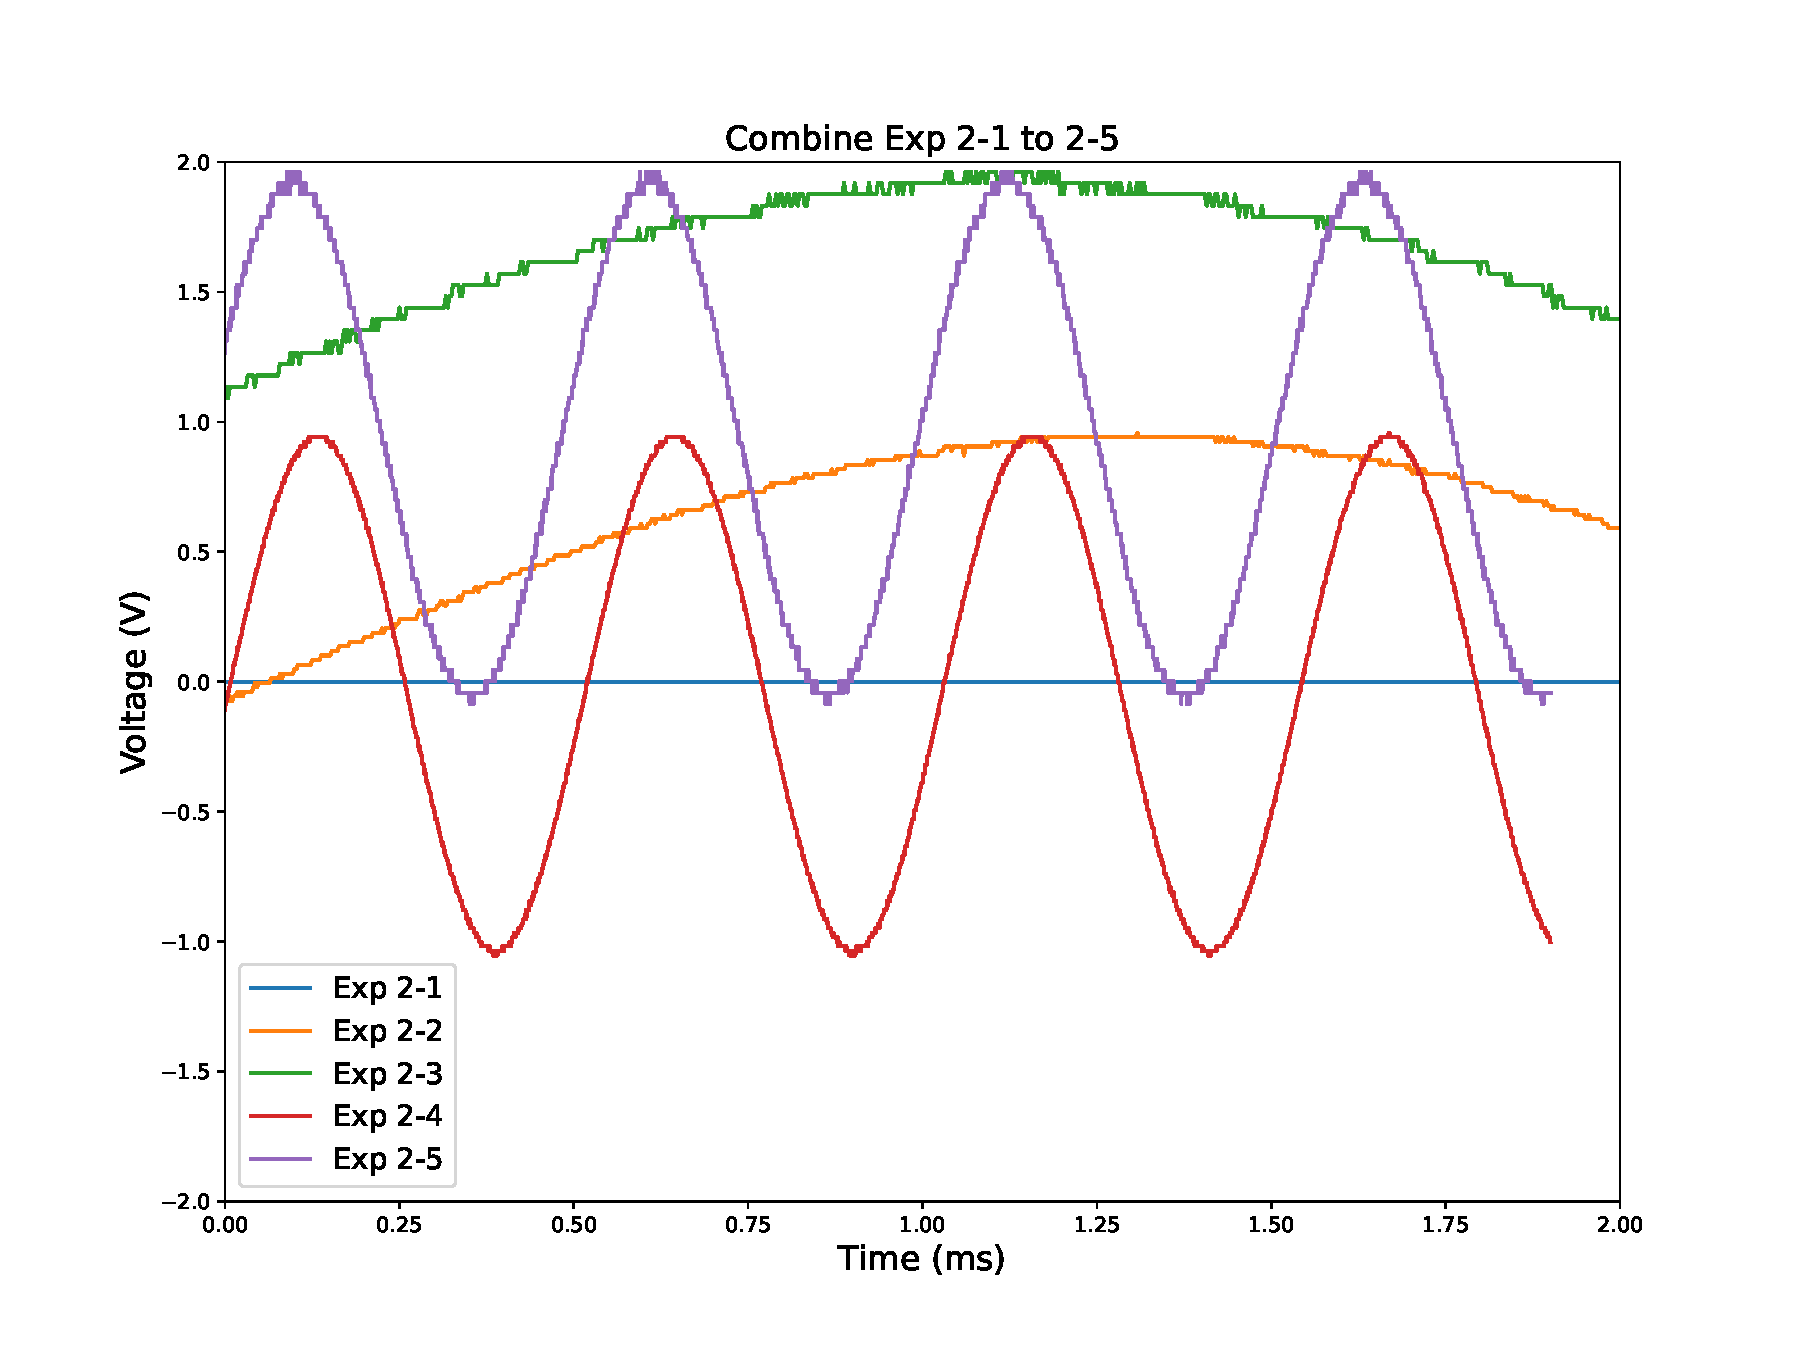
\includegraphics[width=0.9\linewidth]{figures/combine.pdf}
    \caption{The results}
    \label{fig:practice_4_result}
\end{figure}



\clearpage
\section{Analysis and Discussion}\label{sec:discussion}

\subsection{Practice 1}
\hfill

\begin{center}
    \bf Will the mean and standard deviation be the same as the population?
\end{center}

Comparing the initial mean and deviation to the data above (Fig.\ref{fig:actual_1_3}), the two values are not equal.
    
The primary reason for this difference is sampling variability, which means that different samples might lead to different results. Since our samples are random samples based on Gaussian distribution, the number of samples might not be enough to make the two values equal. According to the law of large numbers (LLN), the average of the results obtained from a large number of independent random samples converges to the true value, if it exists. Thus, if we want to make these two values equal, we should raise the sample size.


To testify to the law of large numbers (LLN), we examine how many samples are required to decrease the difference in means and standard deviations, i.e., to check the minimum sample size to make the differences lower than assigned tolerances. 

\begin{equation}
    |\mu_{sample}-\mu_{ideal}|<tolerance
\end{equation}
\begin{equation}
    |\sigma_{sample}-\sigma_{ideal}|<tolerance
\end{equation}
\begin{figure}[h]
    \centering
    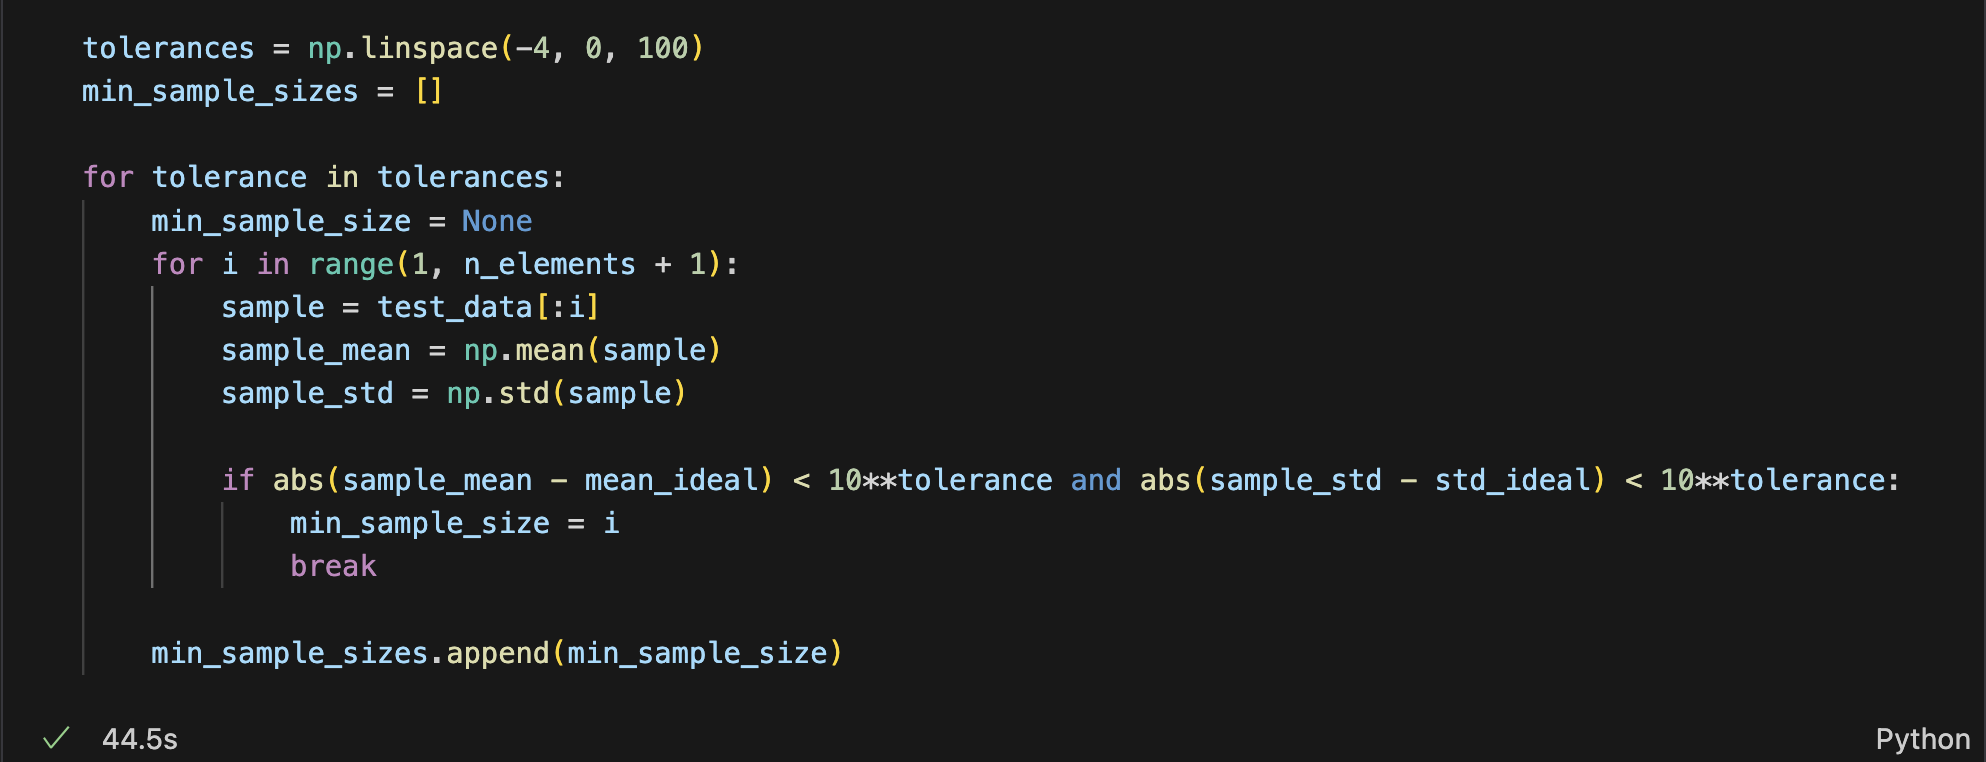
\includegraphics[height=6cm]{figures/code/code_1_6.png}
    \caption{Code to testify law of large numbers}
    \label{fig:code_1_6}
\end{figure}

\clearpage

\begin{figure}[h]
    \centering
    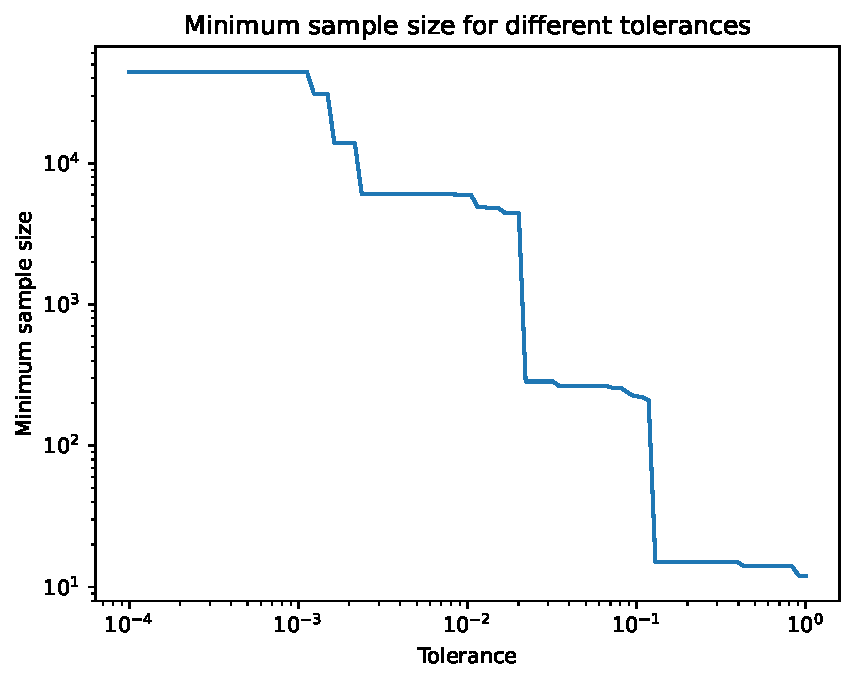
\includegraphics[width=0.7\linewidth]{figures/practice_1_1_tolerance.pdf}
    \caption{Minimum sample sizes required to match the given tolerances}
    \label{fig:practice_1_1_tolerance}
\end{figure}

As we can see in Fig. \ref{fig:practice_1_1_tolerance}, the smaller the given tolerance, the larger the minimum sample sizes needed, confirming the law of large numbers (LLN).

\subsection{Practice 2}
\hfill

This experiment analyzes the statistical characteristics of 50 randomly generated data points with a mean of 0 and a standard deviation of 3. The obtained sample mean is approximately -0.6764, and the standard deviation is around 2.7729.

From the analysis in Fig. \ref{fig:practice_2_1}, 33 data points fall within $\pm$1 standard deviation of the sample mean, accounting for about 66\% of the total data. This is close to the theoretical expectation that approximately 68\% of the data should lie within $\pm$1 standard deviation of the mean. Since the data is randomly generated, experimental results may deviate from theoretical values. To obtain results that more closely align with theoretical expectations, increasing the sample size can help reduce the effect of random errors.

\clearpage



% \begin{figure}[h]
%     \centering
%     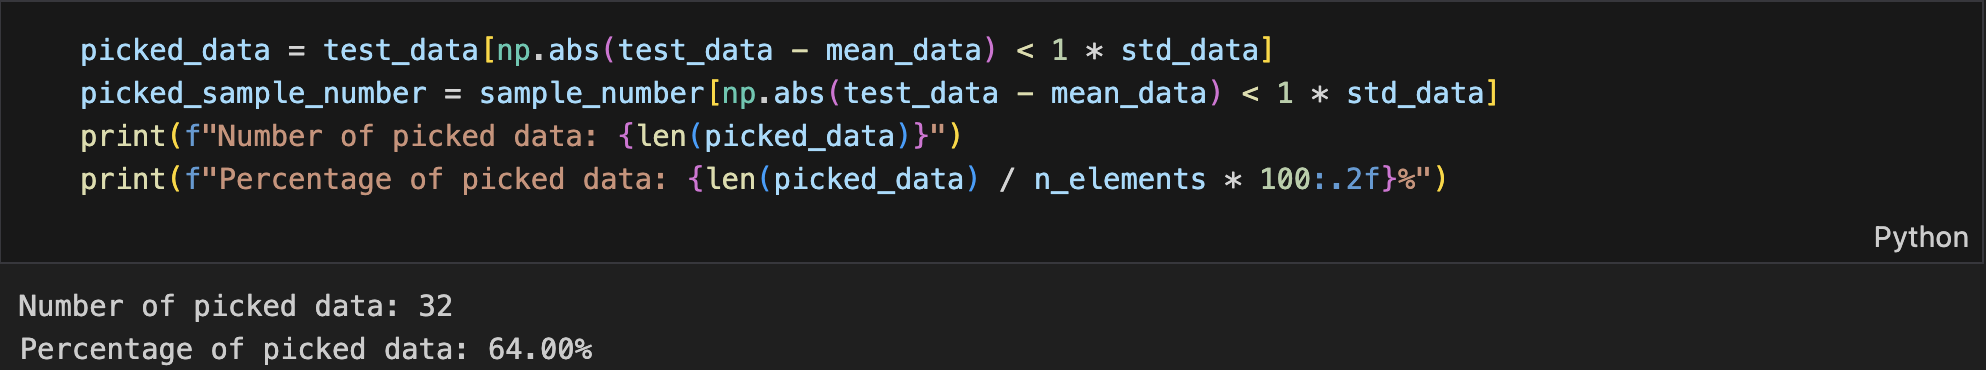
\includegraphics[width=0.9\linewidth]{figures/code/code_2_5.png}
%     \caption{Total number of picked data is 32 and the percentage of picked data is 64\%}
%     \label{fig:code_2_5}
% \end{figure}


\subsection{Practice 3}
\hfill

We add noise to a linear equation and fit the data, where the noise follows a normal distribution with a mean of 0 and a standard deviation of 2. This setting ensures that no outliers appear in the dataset.

Observing the left plot in Fig. \ref{fig:practice_2_1_original}, the linear trend remains evident.

Analysis of Fig. \ref{fig:practice_2_1_residual}:

\begin{enumerate}
    \item Definition of residuals:\\
    The residuals $r_i$ are defined as the difference between the observed value $y_i$ and the predicted value $\hat{y}_i$:
    \begin{equation}
        r_i=y_i-\hat{y}_i
    \end{equation}
    \item The residuals are approximately distributed around 0, indicating that the linear model has a reasonable fitting capability.
    \item Since the noise has a standard deviation of 2, most residuals fall within the range $[-4,4]$, which aligns with our assumptions.
\end{enumerate}

\subsection{Practice 4}
\begin{figure}[h]
    \centering
    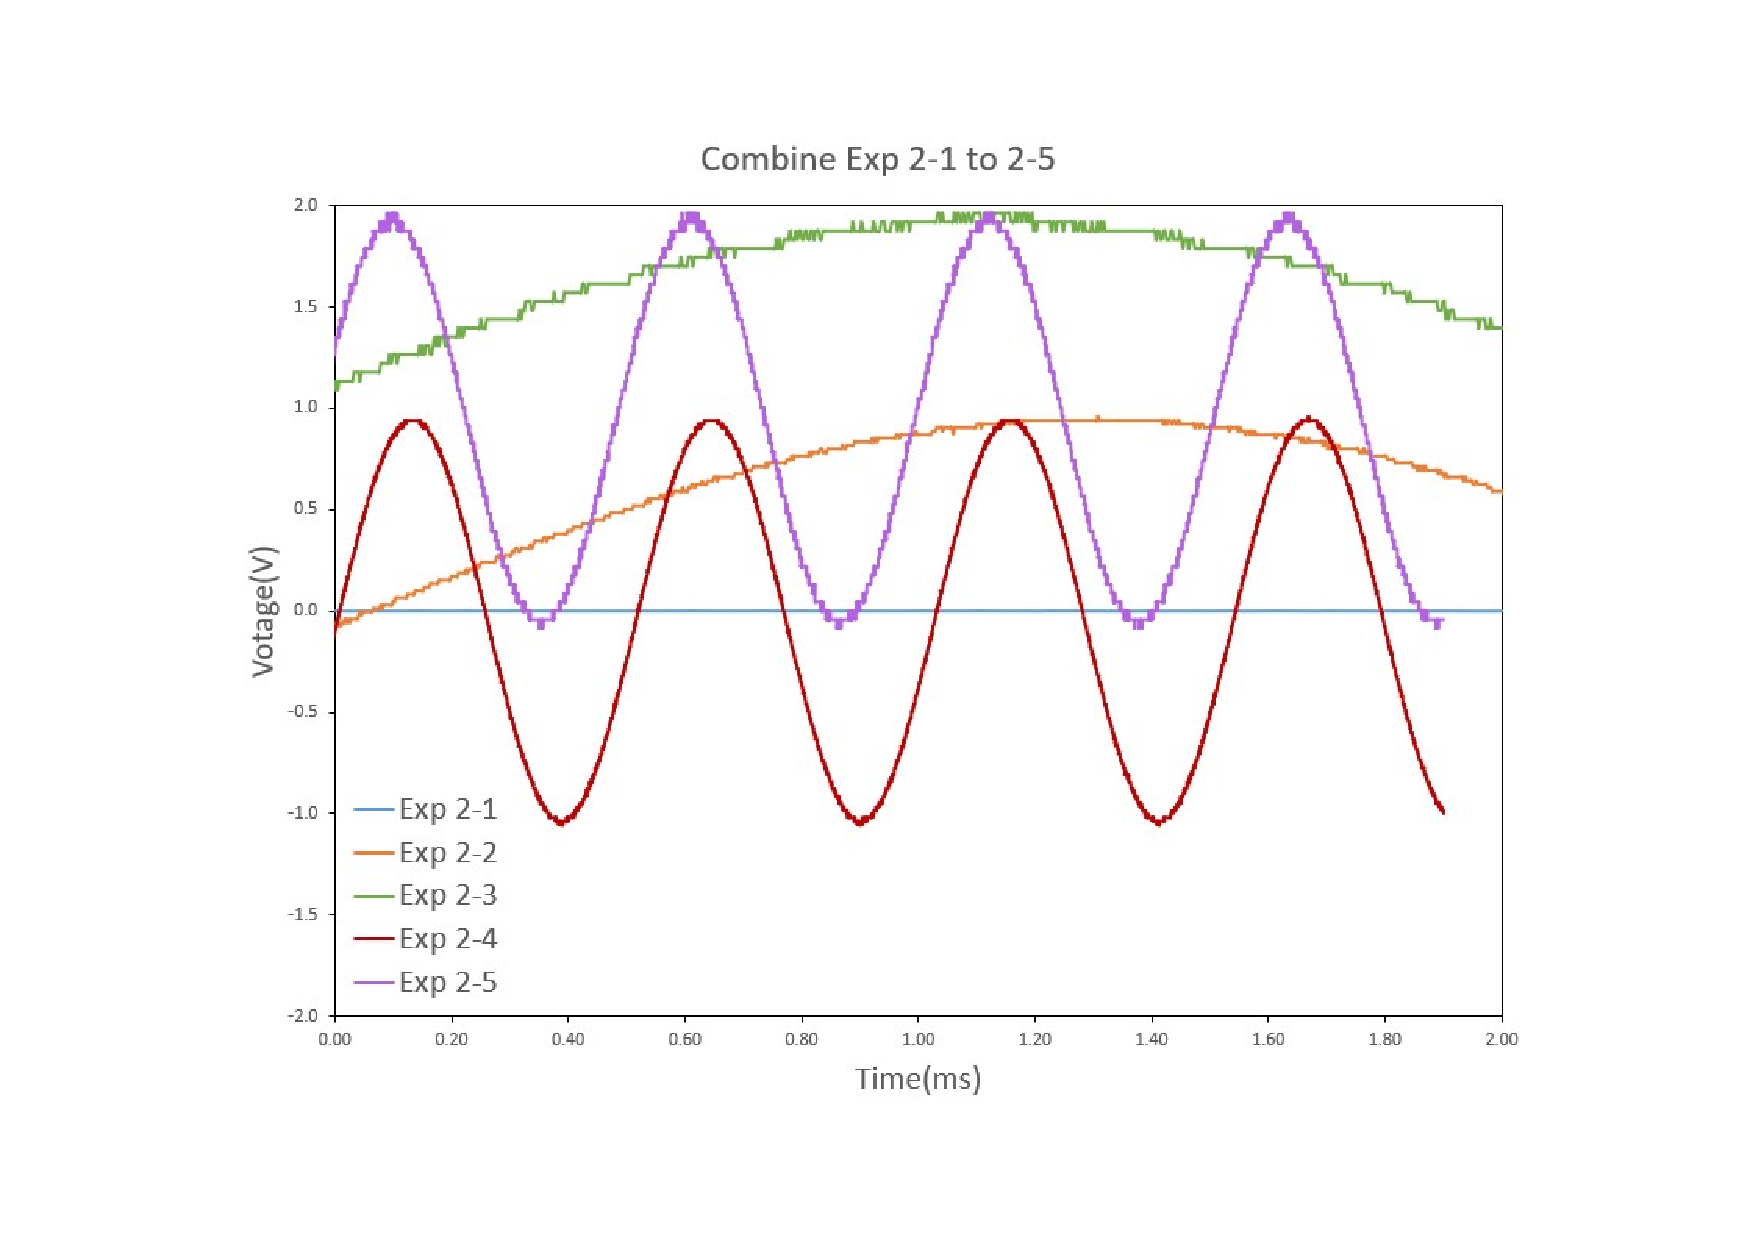
\includegraphics[width=1\linewidth]{figures/Aasfasdsd.pdf}
    \caption{Plot Results from Excel}
    \label{fig:excel}
\end{figure}

The above results were obtained by plotting the same dataset using Excel. Comparing them with the results generated using Python, we can see that they are completely consistent.


\clearpage
\section{Conclusion}\label{sec:conclusion}
\hfill

\indent In this course, we learned how to use Python and explored various data processing tools, including NumPy, Matplotlib, Pandas, SciPy, and Anaconda. With these tools, we were able to efficiently obtain the necessary data and create various types of charts that meet specific requirements using Python.

\indent Throughout the course, we completed several hands-on exercises. Practice 1 focused on analyzing the properties of normal distribution using Python. We imported the numpy and matplotlib.pyplot packages and discussed the differences in mean and standard deviation values. Practice 2 emphasized data visualization, also utilizing numpy and matplotlib.pyplot.

\indent Practice 3 introduced the application of the curve\_fit function, where we learned to plot fitted points and then calculate and plot the residuals. Practice 4 involved reading data from a CSV file and generating a combined chart for Exp 2-1 to 2-5.

\indent In addition to practicing basic Python syntax and applying it to exercises, we also analyzed the results of our data and visualizations, reflecting on how to improve our methods to achieve more accurate outcomes.


\section{Work division}\label{sec:work}
% \hfill

\begin{itemize}
    \item 洪瑜: Analysis, Report
    \item 黃巧涵: Analysis, Report
    \item 洪懌平: Coding, Report
\end{itemize}

\begin{figure}[h]
    \centering
    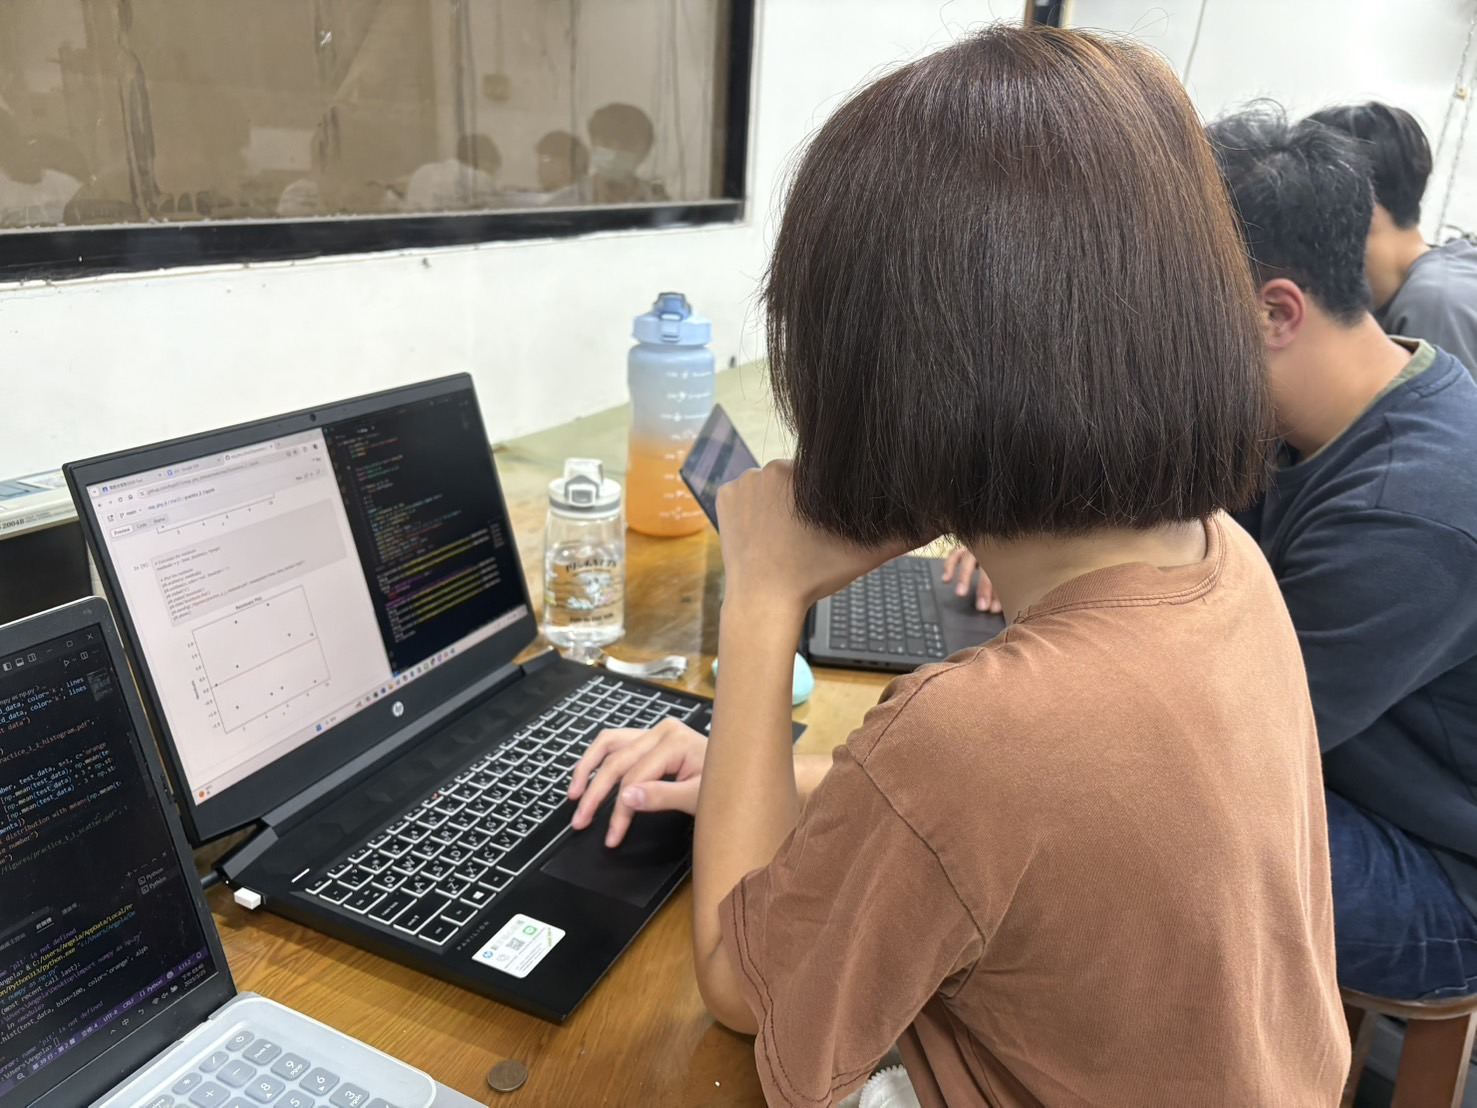
\includegraphics[width=0.30\linewidth]{figures/hyu.jpg}
    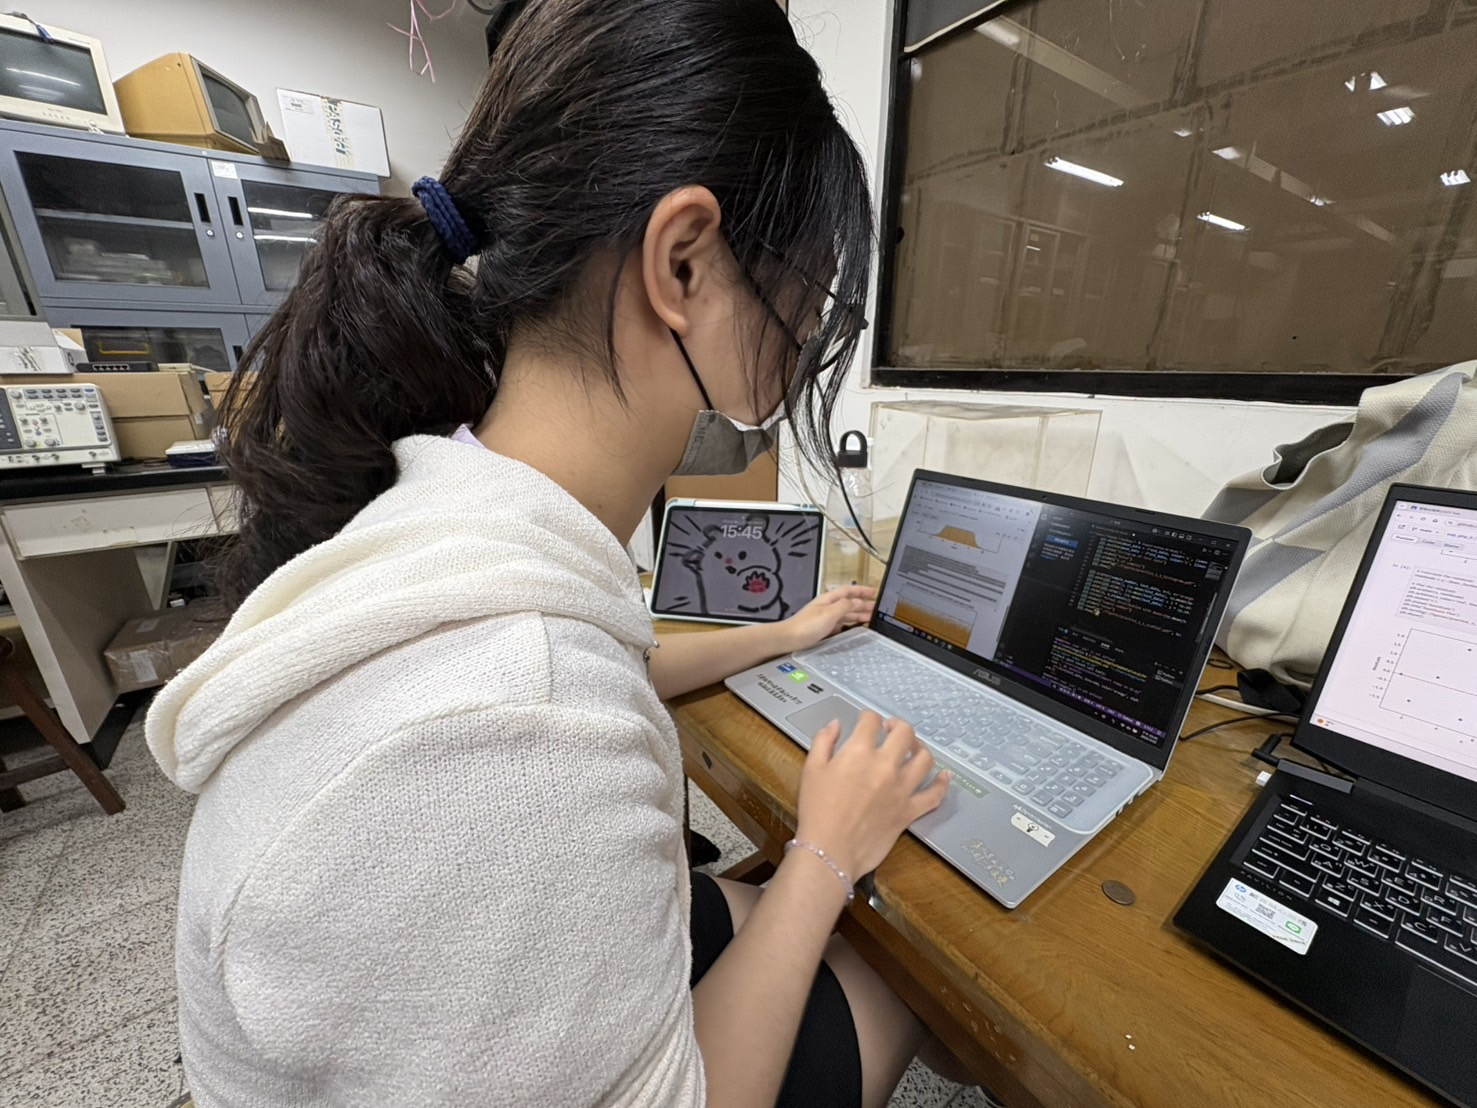
\includegraphics[width=0.30\linewidth]{figures/hch.jpg}
    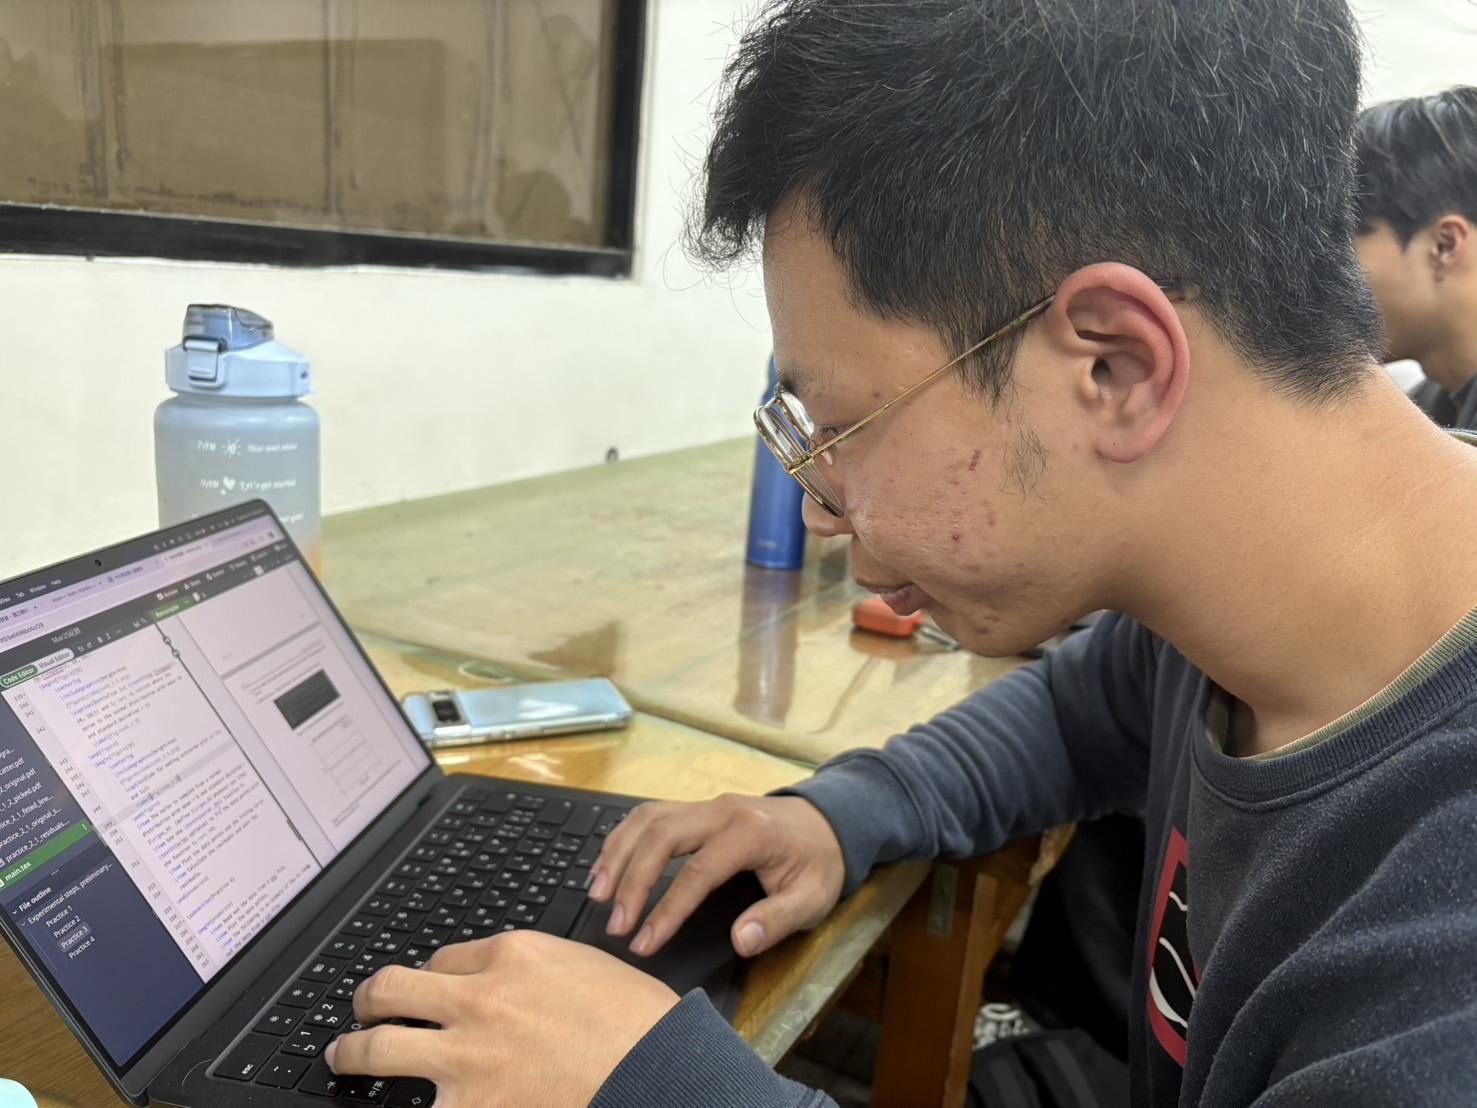
\includegraphics[width=0.30\linewidth]{figures/hyp.jpg}
    \caption{洪瑜(\textit{left}), 黃巧涵(\textit{middle}), and 洪懌平(\textit{right})}
    \label{fig:work}
\end{figure}




\clearpage
\section{Reference}\label{sec:reference}
% \hfill

\begin{itemize}
    \item [1]: The Standard Normal Distribution:\\
    \url{https://www.scribbr.co.uk/stats/the-standard-normal-distribution/}
\end{itemize}


% \clearpage
\section{Appendix}
\hfill

The source codes of these practices can be found at:
\begin{itemize}
    \item \textbf{Practice 1:}\\
    \url{https://github.com/hyp0515/exp_phy_ii/blob/main/mar25/practice_1_1.ipynb}
    \item \textbf{Practice 2:}\\
    \url{https://github.com/hyp0515/exp_phy_ii/blob/main/mar25/practice_1_2.ipynb}
    \item \textbf{Practice 3:}\\
    \url{https://github.com/hyp0515/exp_phy_ii/blob/main/mar25/practice_2_1.ipynb}
    \item \textbf{Practice 4:}\\
    \url{https://github.com/hyp0515/exp_phy_ii/blob/main/mar25/practice_2_2.ipynb}
\end{itemize}


\end{CJK}
\end{document}
